% ============================================================
% borrador_3_Marco_Teorico.tex — Borrador independiente de 3_Marco_Teorico
% Generado automáticamente por compilar_borradores.sh. No editar a mano.
% Compilación: cd Docs/capitulos/3_Marco_Teorico && latexmk -pdf borrador_3_Marco_Teorico.tex
% ============================================================
% ============================================================
% comun/preambulo.tex — Preámbulo unificado para borradores
% Generado automáticamente por compilar_borradores.sh. No editar.
% ============================================================

% ============================================================
%  DOCUMENTO LaTeX
%  Título: Modelo de transformación cuántica variacional de
%          características de cáncer de mama para un sistema
%          híbrido de prediagnóstico
%  Instituto: Instituto Politécnico Nacional — ESCOM
%  TT No. 2026 – B039
% ============================================================

% ------------------------------------------------------------
% PREÁMBULO — paquetes y configuración general
% ------------------------------------------------------------
\documentclass[12pt, letterpaper]{article}
% Codificación y lenguaje
\usepackage[utf8]{inputenc}
\usepackage[T1]{fontenc}
\usepackage[spanish]{babel}
\usepackage{amsmath}
\usepackage{amssymb}

% Tipografía — compatible con pdflatex
\usepackage{mathptmx}  % Times New Roman

% Márgenes y geometría de página
\usepackage[
  top=2cm,
  bottom=2cm,
  left=3cm,
  right=2cm
]{geometry}

% Interlineado
\usepackage{setspace}
\setstretch{1.3}

% Imágenes y gráficos
\usepackage{graphicx}
\graphicspath{{../../}{../}{./}}
\usepackage{float}
\usepackage{adjustbox}

% Hipervínculos y tabla de contenidos
\usepackage{xr-hyper}
\usepackage{hyperref}
\hypersetup{
  colorlinks = true,
  linkcolor  = black,
  urlcolor   = blue,
  citecolor  = black
  }
  
  % Numeración de figuras por subsección
  \usepackage{amsmath}
  \numberwithin{figure}{subsection}
  
  % Tablas
  \usepackage{booktabs}
  \usepackage{array}
  \usepackage{tabularx}
  \usepackage{caption}
  \usepackage{subcaption}
  \usepackage{colortbl}
  \usepackage{xcolor}
  \usepackage{pdflscape}
  \usepackage{pifont}
  \usepackage{longtable}
  
  % Definir checkmark y xmark
  \newcommand{\cmark}{\ding{51}}
  \newcommand{\xmark}{\ding{55}}
  
  % TikZ para elementos gráficos
\usepackage[dvipsnames, table]{xcolor}
\usepackage{tikz}
\usetikzlibrary{arrows.meta, positioning, calc}
\usepackage{amssymb}

\definecolor{colTeal}  {HTML}{0F6E56}
\definecolor{colTealBg}{HTML}{E1F5EE}
\definecolor{colPurp}  {HTML}{534AB7}
\definecolor{colPurpBg}{HTML}{EEEDFE}
\definecolor{colAmber} {HTML}{854F0B}
\definecolor{colAmberBg}{HTML}{FAEEDA}
\definecolor{colCoral} {HTML}{993C1D}
\definecolor{colCoralBg}{HTML}{FAECE7}
\definecolor{colGrayBg}{HTML}{F1EFE8}
\definecolor{colGray}  {HTML}{5F5E5A}

% ── Estilos TikZ ─────────────────────────────────────────
\tikzset{
  blk/.style={
    rectangle, rounded corners=5pt,
    text width=10cm, minimum height=1.1cm,
    align=center, inner sep=6pt,
    font=\small\bfseries,
    draw=#1!60, fill=#1!10
  },
  blkTeal/.style  = {blk=colTeal},
  blkCoral/.style = {blk=colCoral},
  blkAmber/.style = {blk=colAmber},
  blkGray/.style  = {
    rectangle, rounded corners=5pt,
    text width=10cm, minimum height=1.1cm,
    align=center, inner sep=6pt,
    font=\small\bfseries,
    draw=colGray!60, fill=colGrayBg
  },
  cond/.style={
    rectangle, rounded corners=4pt,
    text width=2.3cm, minimum height=1.6cm,
    align=center, inner sep=4pt,
    font=\scriptsize\bfseries,
    draw=colGray!50, fill=colGrayBg
  },
  condQ/.style={
    rectangle, rounded corners=5pt,
    text width=2.5cm, minimum height=1.9cm,
    align=center, inner sep=4pt,
    font=\scriptsize\bfseries,
    draw=colPurp!70, fill=colPurpBg,
    line width=0.8pt
  },
  arr/.style={
    -{Stealth[length=4pt, width=4pt]},
    line width=0.6pt, color=colGray
  }
}

% Encabezados y pies de página personalizados
\usepackage{fancyhdr}


% Espaciado entre párrafos
\usepackage{parskip}
\setlength{\parindent}{0pt}

% Encabezados de sección sin numeración automática en índice
\usepackage{titlesec}

% Bibliografía y citas con hipervínculos
\usepackage{url}
\usepackage[numbers, square]{natbib}   % Citas numéricas estilo [1], [2], etc.
% NOTA: hyperref + natbib hacen que el número sea un hipervínculo automáticamente.

% Líneas divisoras — comandos personalizados
% Uso: \divider          → línea fina al ancho del texto
% Uso: \dividerthick     → línea más gruesa
\newcommand{\divider}{%
  \vspace{0.8em}%
  \noindent\rule{\linewidth}{0.4pt}%
  \vspace{0.8em}%
}
\newcommand{\dividerthick}{%
  \vspace{0.8em}%
  \noindent\rule{\linewidth}{1.2pt}%
  \vspace{0.8em}%
}

% ------------------------------------------------------------
% INICIO DEL DOCUMENTO
% ------------------------------------------------------------

% ============================================================
% preambulo_extra.tex — paquetes que los capítulos nuevos necesitan y que el preámbulo de
% Technical_Report.tex todavía no carga. Al integrar, copiar estas líneas antes de \begin{document}.
% ============================================================
\usepackage{listings}
\renewcommand{\lstlistingname}{Listado}
\renewcommand{\lstlistlistingname}{Índice de listados}
\lstdefinestyle{tt}{
  language=Python,
  basicstyle=\ttfamily\scriptsize,
  keywordstyle=\color{blue!60!black}\bfseries,
  commentstyle=\color{gray}\itshape,
  stringstyle=\color{green!40!black},
  numbers=left, numberstyle=\tiny\color{gray}, numbersep=6pt,
  frame=single, rulecolor=\color{gray!50},
  breaklines=true, breakatwhitespace=false, columns=fullflexible, keepspaces=true,
  showstringspaces=false, tabsize=4, captionpos=t,
  firstline=2,   % la línea 1 de cada archivo de Docs/codigo/ es la cabecera «# fuente: …»
  inputencoding=utf8, extendedchars=true,
  literate=
    {á}{{\'a}}1 {é}{{\'e}}1 {í}{{\'i}}1 {ó}{{\'o}}1 {ú}{{\'u}}1
    {Á}{{\'A}}1 {É}{{\'E}}1 {Í}{{\'I}}1 {Ó}{{\'O}}1 {Ú}{{\'U}}1
    {ñ}{{\~n}}1 {Ñ}{{\~N}}1 {ü}{{\"u}}1 {Ü}{{\"U}}1 {ö}{{\"o}}1
    {¿}{{?`}}1 {¡}{{!`}}1 {«}{{\guillemotleft}}1 {»}{{\guillemotright}}1
    {θ}{{$\theta$}}1 {π}{{$\pi$}}1 {γ}{{$\gamma$}}1 {λ}{{$\lambda$}}1 {ρ}{{$\rho$}}1
    {σ}{{$\sigma$}}1 {μ}{{$\mu$}}1 {α}{{$\alpha$}}1 {β}{{$\beta$}}1 {ψ}{{$\psi$}}1 {φ}{{$\phi$}}1
    {Δ}{{$\Delta$}}1 {Σ}{{$\Sigma$}}1 {Ψ}{{$\Psi$}}1
    {⟨}{{$\langle$}}1 {⟩}{{$\rangle$}}1 {≤}{{$\le$}}1 {≥}{{$\ge$}}1 {≈}{{$\approx$}}1 {≠}{{$\ne$}}1
    {→}{{$\to$}}1 {←}{{$\leftarrow$}}1 {×}{{$\times$}}1 {·}{{$\cdot$}}1 {±}{{$\pm$}}1 {√}{{$\surd$}}1
    {∞}{{$\infty$}}1 {∈}{{$\in$}}1 {ᵢ}{{$_i$}}1 {ⱼ}{{$_j$}}1 {²}{{$^2$}}1 {³}{{$^3$}}1 {⁻}{{$^-$}}1 {¹}{{$^1$}}1
    {—}{{---}}1 {–}{{--}}1 {’}{{'}}1 {‘}{{`}}1 {“}{{``}}1 {”}{{''}}1 {…}{{\ldots}}1 {°}{{$^\circ$}}1 {‖}{{$\|$}}1
}

\externaldocument{../_build/externo_3_Marco_Teorico}

\begin{document}

\setcounter{section}{2}

% ---
% Reemplaza líneas 980-985 de Docs/Technical_Report.tex
% Decisiones: N/A (estructura base)
% ---

\newpage
\section{Marco Teórico}

% ---
% Reemplaza líneas 986-1035 de Docs/Technical_Report.tex
% Decisiones: N/A (sin cambio)
% ---

\subsection{Fundamentos de computación cuántica}

El presente bloque introduce los conceptos y formalismos matemáticos de la computación cuántica que sustentan la implementación del circuito variacional desarrollado en este trabajo. La referencia estándar para esta sección es Nielsen y Chuang \cite{nielsen2010quantum}.

% -----------------------------------------------------------
\subsubsection{El qubit como unidad de información cuántica}
% -----------------------------------------------------------

La unidad fundamental de información en la computación cuántica es el \textit{qubit} (quantum bit). A diferencia de un bit clásico, que solo puede tomar los valores 0 o 1, un qubit puede encontrarse en una \textit{superposición} de ambos estados simultáneamente. Formalmente, el estado de un qubit se representa como un vector unitario en un espacio de Hilbert bidimensional $\mathcal{H} = \mathbb{C}^2$:

\begin{equation}
    |\psi\rangle = \alpha|0\rangle + \beta|1\rangle, 
    \quad \alpha, \beta \in \mathbb{C}, 
    \quad |\alpha|^2 + |\beta|^2 = 1
    \label{eq:qubit}
\end{equation}

\noindent donde $|0\rangle$ y $|1\rangle$ son los vectores de la base computacional estándar, análogos a los estados 0 y 1 clásicos:

\begin{equation}
    |0\rangle = \begin{pmatrix} 1 \\ 0 \end{pmatrix}, \qquad
    |1\rangle = \begin{pmatrix} 0 \\ 1 \end{pmatrix}
    \label{eq:basis}
\end{equation}

\noindent Los coeficientes $\alpha$ y $\beta$ son \textit{amplitudes de probabilidad}: al medir el qubit, se obtiene el estado $|0\rangle$ con probabilidad $|\alpha|^2$ y el estado $|1\rangle$ con probabilidad $|\beta|^2$. La medición es irreversible y colapsa el estado a uno de los dos valores de la base.

La representación geométrica estándar de un qubit es la 
\textit{esfera de Bloch}, que parametriza el estado general de 
un qubit (salvo fase global) mediante dos ángulos reales:

\begin{equation}
    |\psi\rangle = \cos\!\left(\frac{\theta}{2}\right)|0\rangle 
    + e^{i\varphi}\sin\!\left(\frac{\theta}{2}\right)|1\rangle,
    \quad \theta \in [0, \pi],\; \varphi \in [0, 2\pi)
    \label{eq:bloch}
\end{equation}

\noindent donde $\theta$ determina la mezcla entre $|0\rangle$ y $|1\rangle$, y $\varphi$ es la fase relativa entre ambos. Esta parametrización es fundamental para entender las compuertas de rotación que conforman los circuitos variacionales del presente trabajo \cite{nielsen2010quantum} (figura~\ref{fig:bloch}).

\begin{figure}[t]
    \centering
    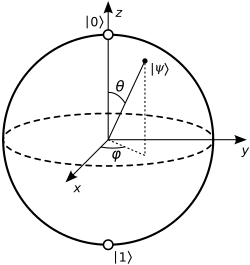
\includegraphics[width=0.3\textwidth]{Figures/Figura_3_1_1.png}
    \caption{Esfera de Bloch: representación geométrica de un qubit. 
    El estado $|\psi\rangle$ se representa como un punto en la 
    superficie de la esfera, determinado por los ángulos $\theta$ y 
    $\varphi$.}
    \label{fig:bloch}
\end{figure}

% ---
% Reemplaza líneas 1037-1092 de Docs/Technical_Report.tex
% Decisiones: N/A (sin cambio)
% ---

\subsubsection{Compuertas cuánticas de un qubit}
% -----------------------------------------------------------

Las operaciones sobre qubits se realizan mediante \textit{compuertas cuánticas}, representadas por matrices unitarias $U \in \mathbb{C}^{2\times 2}$ que satisfacen $UU^\dagger = I$. La unitariedad garantiza la reversibilidad de la operación y la conservación de la norma del estado. Las compuertas más relevantes para los circuitos variacionales son las rotaciones parametrizadas alrededor de los ejes de la esfera de Bloch \cite{nielsen2010quantum}:

\begin{equation}
    R_X(\theta) = e^{-i\frac{\theta}{2}X} = 
    \begin{pmatrix} 
        \cos\frac{\theta}{2}  & -i\sin\frac{\theta}{2} \\ 
        -i\sin\frac{\theta}{2} & \cos\frac{\theta}{2} 
    \end{pmatrix}
    \label{eq:rx}
\end{equation}

\begin{equation}
    R_Y(\theta) = e^{-i\frac{\theta}{2}Y} = 
    \begin{pmatrix} 
        \cos\frac{\theta}{2}  & -\sin\frac{\theta}{2} \\ 
        \sin\frac{\theta}{2}  & \cos\frac{\theta}{2} 
    \end{pmatrix}
    \label{eq:ry}
\end{equation}

\begin{equation}
    R_Z(\theta) = e^{-i\frac{\theta}{2}Z} = 
    \begin{pmatrix} 
        e^{-i\frac{\theta}{2}} & 0 \\ 
        0 & e^{i\frac{\theta}{2}} 
    \end{pmatrix}
    \label{eq:rz}
\end{equation}

\noindent donde $X$, $Y$ y $Z$ son las matrices de Pauli:

\begin{equation}
    X = \begin{pmatrix} 0 & 1 \\ 1 & 0 \end{pmatrix}, \quad
    Y = \begin{pmatrix} 0 & -i \\ i & 0 \end{pmatrix}, \quad
    Z = \begin{pmatrix} 1 & 0 \\ 0 & -1 \end{pmatrix}
    \label{eq:pauli}
\end{equation}

Estas compuertas de rotación son los bloques de construcción del ansatz variacional implementado en Qiskit, donde los ángulos $\theta$ son los parámetros entrenables del circuito. La compuerta de Hadamard, definida como:

\begin{equation}
    H = \frac{1}{\sqrt{2}}\begin{pmatrix} 1 & 1 \\ 1 & -1 
    \end{pmatrix}
    \label{eq:hadamard}
\end{equation}

\noindent transforma el estado base $|0\rangle$ en la 
superposición uniforme 
$\frac{1}{\sqrt{2}}(|0\rangle + |1\rangle)$, y es 
ampliamente utilizada como compuerta de inicialización en 
circuitos cuánticos.

% ---
% Reemplaza líneas 1093-1138 de Docs/Technical_Report.tex
% Decisiones: N/A (sin cambio)
% ---

\subsubsection{Sistemas de múltiples qubits y entrelazamiento}
% -----------------------------------------------------------

El estado de un sistema de $n$ qubits se describe mediante el producto tensorial de los espacios de Hilbert individuales:

\begin{equation}
    \mathcal{H}^{\otimes n} = 
    \underbrace{\mathbb{C}^2 \otimes \mathbb{C}^2 \otimes 
    \cdots \otimes \mathbb{C}^2}_{n}, 
    \quad \dim(\mathcal{H}^{\otimes n}) = 2^n
    \label{eq:tensor}
\end{equation}

\noindent El estado general de $n$ qubits es una superposición 
de los $2^n$ estados de la base computacional 
$\{|0\cdots0\rangle, |0\cdots1\rangle, \ldots, 
|1\cdots1\rangle\}$:

\begin{equation}
    |\Psi\rangle = \sum_{k=0}^{2^n - 1} c_k |k\rangle, 
    \quad c_k \in \mathbb{C}, 
    \quad \sum_{k=0}^{2^n-1} |c_k|^2 = 1
    \label{eq:multiQubit}
\end{equation}

El \textit{entrelazamiento cuántico} es la propiedad por la cual el estado de un sistema de múltiples qubits no puede factorizarse como el producto tensorial de estados individuales. Un estado entrelazado no tiene representación separable y exhibe correlaciones entre qubits que no tienen análogo clásico \cite{nielsen2010quantum}. La compuerta estándar para generar entrelazamiento es la \textit{compuerta CNOT} (Controlled-NOT), que opera sobre dos qubits: un qubit de control $c$ y un qubit objetivo $t$, aplicando una negación al objetivo condicionada al estado del control:

\begin{equation}
    \text{CNOT} = 
    \begin{pmatrix} 
        1 & 0 & 0 & 0 \\ 
        0 & 1 & 0 & 0 \\ 
        0 & 0 & 0 & 1 \\ 
        0 & 0 & 1 & 0 
    \end{pmatrix}
    \label{eq:cnot}
\end{equation}

\noindent La combinación de compuertas de rotación de un qubit 
y compuertas CNOT es suficiente para aproximar cualquier 
operación unitaria sobre $n$ qubits, propiedad conocida como 
\textit{universalidad} \cite{nielsen2010quantum}. Esta 
combinación es precisamente la que estructura el ansatz 
variacional RealAmplitudes utilizado en el presente trabajo.

% ---
% Reemplaza líneas 1139-1190 de Docs/Technical_Report.tex
% Decisiones: D-014, D-040, H-019, H-052
% ---

\subsubsection{Medición y valores de expectativa}

La medición en computación cuántica extrae información clásica del estado cuántico
al precio de colapsar la superposición. Para un observable $\hat{O}$ representado
por un operador hermítico, el valor de expectativa cuantifica el promedio estadístico
obtenido al medir dicho observable sobre un ensamble de estados idénticos $|\psi\rangle$:
\begin{equation}
  \langle \hat{O} \rangle = \langle \psi | \hat{O} | \psi \rangle.
  \label{eq:expectation}
\end{equation}
En el presente trabajo, los observables corresponden a las matrices
de Pauli $Z$ aplicadas a cada qubit individual $i \in \{1, \dots, n\}$. Su valor
de expectativa está en el intervalo $[-1, 1]$:
\begin{equation}
  \langle Z_i \rangle = \langle \psi | Z_i | \psi \rangle \in [-1, 1],
  \label{eq:expZ}
\end{equation}
donde $\langle Z_i \rangle = +1$ denota el estado computacional $|0\rangle$,
$\langle Z_i \rangle = -1$ denota el estado $|1\rangle$, y valores intermedios
describen superposiciones coherentes o mezclas estadísticas. El vector ordenado de
expectativas:
\begin{equation}
  \mathbf{e}_Z = \bigl(\langle Z_1 \rangle, \langle Z_2 \rangle, \dots, \langle Z_n \rangle\bigr)^\top \in [-1, 1]^n
  \label{eq:expZ_vector}
\end{equation}
resume la proyección del estado cuántico sobre cada qubit.

En un dispositivo físico cuántico, $\langle Z_i \rangle$ no se mide de forma
directa sino que se estima mediante el promedio de $n_{\text{shots}}$ mediciones
proyectivas independientes. Dado que los autovalores de $Z_i$ son $\pm 1$, cada disparo da $\pm 1$ con probabilidad $P(+1) = (1+\langle Z_i\rangle)/2$, de modo que la varianza de un disparo individual es $1-\langle Z_i\rangle^2$. La varianza del estimador empírico
$\hat{Z}_i = \frac{1}{n_{\text{shots}}} \sum_{s=1}^{n_{\text{shots}}} z_i^{(s)}$
está determinada exactamente por:
\begin{equation}
  \operatorname{Var}(\hat{Z}_i) = \frac{1 - \langle Z_i \rangle^2}{n_{\text{shots}}}.
  \label{eq:shot_noise_variance}
\end{equation}
La dispersión muestral es máxima cuando el estado es puramente ecuatorial
($\langle Z_i \rangle = 0$, varianza $1/n_{\text{shots}}$) y se anula si el qubit
se halla en un autoestado de la base computacional ($\langle Z_i \rangle = \pm 1$).

El núcleo de fidelidad cuántica, $K_Q(\mathbf{x}, \mathbf{x}') = |\langle \phi(\mathbf{x}) | \phi(\mathbf{x}') \rangle|^2$,
se estima en hardware de otra forma: se implementa el circuito de
\textit{compute-uncompute} $U^\dagger(\mathbf{x}') U(\mathbf{x})$ sobre el estado
$|0\rangle^{\otimes n}$ y se cuenta la frecuencia con la que se registra
la cadena nula $|0\dots 0\rangle$. Por lo tanto, la estimación del kernel en hardware
es un proceso binomial con probabilidad de éxito $p = K_Q$, cuya
varianza muestral es $K_Q(1 - K_Q)/n_{\text{shots}}$.

En la metodología principal del presente trabajo, con objeto de evaluar las
propiedades geométricas de las representaciones sin el ruido
que introduce un número finito de disparos, los valores de
expectativa y las matrices de fidelidad se evalúan analíticamente en simulación a
partir del vector de estado exacto (\textit{statevector}). El impacto empírico y
analítico de la cota finita de disparos ($n_{\text{shots}}$) se analiza de forma
explícita en el módulo de restricciones del simulador (M8).

% ---
% Reemplaza líneas 1191-1229 de Docs/Technical_Report.tex
% Decisiones: N/A (sin cambio)
% ---

\subsection{Circuitos cuánticos variacionales y 
            \textit{quantum embeddings}}

% -----------------------------------------------------------
\subsubsection{Circuitos cuánticos parametrizados (PQC)}
% -----------------------------------------------------------

Un \textit{circuito cuántico parametrizado} (PQC, por sus
siglas en inglés) es un circuito cuántico cuyas compuertas
dependen de un conjunto de parámetros reales
$\boldsymbol{\theta} \in \mathbb{R}^m$ que pueden ajustarse
mediante optimización clásica \cite{cerezo2021variational}.
Un \textit{circuito cuántico variacional} (VQC) es un tipo
específico de PQC que combina un bloque de codificación de
datos $U(\mathbf{x})$ con un bloque variacional entrenable
$W(\boldsymbol{\theta})$, produciendo el estado cuántico:

\begin{equation}
  |\psi(\mathbf{x}, \boldsymbol{\theta})\rangle =
  W(\boldsymbol{\theta})\,U(\mathbf{x})\,
  |0\rangle^{\otimes n}
  \label{eq:vqc_state}
\end{equation}

\noindent donde $n$ es el número de qubits,
$U(\mathbf{x})$ es el \textit{feature map} cuántico que
codifica el vector de características clásico
$\mathbf{x} \in \mathbb{R}^k$ en el estado cuántico inicial,
y $W(\boldsymbol{\theta})$ es el \textit{ansatz} variacional
que introduce correlaciones entre qubits mediante compuertas
entrenables \cite{Schuld2019QuantumML}.

La arquitectura VQC es la más adecuada para el régimen NISQ
actual porque mantiene profundidades de circuito moderadas
y es diferenciable de extremo a extremo mediante el método
de \textit{parameter-shift}, descrito en la
sección~\ref{sec:parameter_shift}.

% ---
% Reemplaza líneas 1230-1274 de Docs/Technical_Report.tex
% Decisiones: N/A (sin cambio)
% ---

\subsubsection{El \textit{feature map} como mapeo no lineal al espacio de Hilbert}
\label{sec:feature_map}
% -----------------------------------------------------------

El bloque $U(\mathbf{x})$ define un mapeo no lineal:

\begin{equation}
  \phi: \mathbb{R}^k \rightarrow \mathcal{H}, \qquad
  \mathbf{x} \mapsto |\phi(\mathbf{x})\rangle =
  U(\mathbf{x})\,|0\rangle^{\otimes n}
  \label{eq:feature_map}
\end{equation}

\noindent donde $\mathcal{H} = \mathbb{C}^{2^n}$ es el
espacio de Hilbert del sistema de $n$ qubits, de dimensión
$2^n$. Como se argumentó en la sección del planteamiento
del problema, este espacio no es simplemente una versión
ampliada del espacio clásico de entrada: su geometría está
determinada por productos internos cuánticos
$\langle\phi(\mathbf{x})|\phi(\mathbf{x}')\rangle$, no por
distancias euclidianas. Con compuertas de entrelazamiento,
el mapeo $\phi$ hace depender el estado de productos de pares
de componentes de $\mathbf{x}$ además de cada componente por
separado \cite{Schuld2019QuantumML, havlicek2019supervised}; si
la geometría resultante aporta separabilidad frente a un kernel
clásico es una pregunta empírica, que es la que aborda este trabajo.
% Corregido el 2026-10-19 (auditoría A5-1): decía «correlaciones de orden superior que los métodos
% clásicos no capturan», en contradicción con §2.1.3 y §3.2.4 (interacciones de dos cuerpos como máximo).

Este mapeo define implícitamente un \textit{kernel cuántico}:

\begin{equation}
  k_Q(\mathbf{x}, \mathbf{x}') =
  \left|\langle\phi(\mathbf{x})|\phi(\mathbf{x}')\rangle
  \right|^2 =
  \left|\langle 0|^{\otimes n}\,U^\dagger(\mathbf{x}')\,
  U(\mathbf{x})\,|0\rangle^{\otimes n}\right|^2
  \label{eq:quantum_kernel}
\end{equation}

\noindent La elección del \textit{feature map} $U(\mathbf{x})$
determina completamente la geometría del espacio de
representación y, con ello, la capacidad del sistema para
separar las clases en ese espacio. En el presente trabajo
se comparan dos diseños de \textit{feature map}:
\textit{ZZFeatureMap} y \textit{PauliFeatureMap},
descritos a continuación.

% ---
% Reemplaza líneas 1275-1346 de Docs/Technical_Report.tex
% Decisiones: D-031, H-031
% ---

\subsubsection{\textit{ZZFeatureMap}: evolución de Pauli-Z de segundo orden}

El \textit{ZZFeatureMap} es un circuito de evolución de
Pauli-Z de segundo orden introducido por Havlíček et al.
\cite{havlicek2019supervised} y disponible en Qiskit como
\texttt{zz\_feature\_map}.
Para $n$ qubits y $r$ repeticiones (\texttt{reps}),
el circuito implementa el unitario:

\begin{equation}
  U_{\text{ZZ}}(\mathbf{x}) =
  \left[\mathcal{U}_\Phi(\mathbf{x})\,H^{\otimes n}
  \right]^r
  \label{eq:zzfeaturemap}
\end{equation}

\noindent donde $H^{\otimes n}$ es la capa de compuertas
de Hadamard que inicializa la superposición uniforme, y
$\mathcal{U}_\Phi(\mathbf{x})$ es el bloque de codificación
de datos definido por\footnote{Havlíček et al. y la documentación de Qiskit escriben $+i$; el circuito de Qiskit implementa $-i$, que produce el estado complejo conjugado. El kernel de fidelidad y los valores esperados de este trabajo no dependen de esa elección.}:

\begin{equation}
  \mathcal{U}_\Phi(\mathbf{x}) =
  \exp\!\left(-i \sum_{S \subseteq [n],\,|S|\leq 2}
  \phi_S(\mathbf{x})\,\bigotimes_{j \in S} Z_j\right)
  \label{eq:Uphi}
\end{equation}

\noindent Los coeficientes $\phi_S(\mathbf{x})$ codifican
los datos clásicos en el hamiltoniano de evolución:

\begin{equation}
  \phi_{\{i\}}(\mathbf{x}) = x_i, \qquad
  \phi_{\{i,j\}}(\mathbf{x}) =
  (\pi - x_i)(\pi - x_j)
  \label{eq:phi_coefficients}
\end{equation}

Como $e^{-i\phi Z} = \operatorname{diag}(e^{-i\phi}, e^{i\phi})$, cada término introduce una fase
relativa $2\phi_S$ entre las componentes del estado. Por eso el circuito de Qiskit aplica
compuertas de fase $P(2x_i)$ y $P\bigl(2(\pi-x_i)(\pi-x_j)\bigr)$: el factor 2 corresponde al
parámetro \texttt{alpha} de la función, cuyo valor por defecto es 2. Con $x_i\in[0,\pi]$, la fase
relativa propia recorre la circunferencia una vez.

\noindent El término de un qubit $\phi_{\{i\}}$ codifica
cada característica $x_i$ como una rotación alrededor del
eje $Z$. El término de dos qubits $\phi_{\{i,j\}}$
introduce \textit{entrelazamiento} entre pares de qubits
que codifica las interacciones de segundo orden entre
características, operando mediante la compuerta:

\begin{equation}
  e^{i\,\phi_{\{i,j\}}(\mathbf{x})\,Z_i Z_j} =
  \text{CNOT}_{i \to j}\;
  e^{i\,\phi_{\{i,j\}}(\mathbf{x})\,Z_j}\;
  \text{CNOT}_{i \to j}
  \label{eq:zz_gate}
\end{equation}

\noindent Esta capacidad de capturar interacciones de segundo
orden entre pares de características es la razón por la que
el ZZFeatureMap es uno de los métodos
de codificación de datos más utilizados en tareas de
clasificación cuántica, dada su capacidad para enriquecer la
expresividad del espacio de características cuántico y la
dificultad de simularlo clásicamente. 

Es importante señalar que en Qiskit 2.x el uso de la clase
\texttt{ZZFeatureMap} está marcado como obsoleto
(\textit{deprecated}) a favor de la función
\texttt{zz\_feature\_map()}, que retorna un
\texttt{QuantumCircuit} estándar \cite{ibmquantum2024docs}.
En el presente trabajo se utiliza la función actualizada
compatible con Qiskit 2.x.

% ---
% Reemplaza líneas 1347-1390 de Docs/Technical_Report.tex
% Decisiones: D-031, H-012, H-034
% ---

\subsubsection{\textit{PauliFeatureMap}: generalización por elección de los operadores de Pauli}

El circuito \textit{PauliFeatureMap} constituye la generalización del esquema de
Havl{\'{\i}}{\v{c}}ek et al. que permite seleccionar subconjuntos arbitrarios de
operadores de Pauli ($X$, $Y$, $Z$) en el bloque unitario de codificación. El operador
adopta la forma general:
\begin{equation}
  U_{\text{Pauli}}(\mathbf{x}) = \left[\mathcal{U}_\Phi^{(P)}(\mathbf{x})\,H^{\otimes n}\right]^r,
  \label{eq:paulifeaturemap}
\end{equation}
donde el generador diagonal o no diagonal se define a partir de una familia de cadenas
de Pauli $\{P_S\}$:
\begin{equation}
  \mathcal{U}_\Phi^{(P)}(\mathbf{x}) = \prod_{P \in \mathcal{P}}
  \exp\!\left(-i \sum_{S} \phi_S(\mathbf{x})\,\bigotimes_{j \in S} P_j\right),
  \label{eq:pauli_expansion}
\end{equation}
donde $\mathcal{P}$ es la lista de cadenas de Pauli elegida, en el orden en que se aplican. Si los
términos no conmutan, como $Y$ y $ZZ$, el bloque es un producto de exponenciales y no una
sola exponencial: en C5 se aplica primero $\exp\bigl(-i\sum_i x_i Y_i\bigr)$ y después
$\exp\bigl(-i\sum_{i<j}(\pi-x_i)(\pi-x_j)Z_iZ_j\bigr)$.
En el presente trabajo, la condición experimental C5 se define formalmente como
\texttt{pauli\_feature\_map(paulis=['Y', 'ZZ'], reps=1)}, manteniendo el mismo número
de qubits ($k = 12$) e idéntica conectividad de entrelazamiento de segundo orden
($ZZ$) que el mapa C4 (\texttt{zz\_feature\_map}). La
comparación entre C4 y C5 aísla con precisión el efecto de sustituir el eje de rotación
de la codificación de primer orden (eje $Z$ frente a eje $Y$), preservando
inalterada la estructura del entrelazamiento de dos cuerpos.

La elección de operadores de Pauli en la codificación de un solo qubit tiene consecuencias
geométricas sobre la esfera de Bloch:
\begin{enumerate}
  \item \textbf{El término en $X$ no codifica nada:} Tras la capa inicial de Hadamard,
        el estado del registro se encuentra en $|+\rangle^{\otimes n} = \left(\frac{|0\rangle + |1\rangle}{\sqrt{2}}\right)^{\otimes n}$.
        Dado que el estado $|+\rangle$ es un autoestado del operador de Pauli $X$ con
        autovalor $+1$ ($X|+\rangle = |+\rangle$), la aplicación del operador unitario de
        evolución bajo $X$ satisface:
        \begin{equation}
          e^{-i\,\phi(x_i)\,X}|+\rangle = e^{-i\,\phi(x_i)}\,|+\rangle.
          \label{eq:x_eigenstate_phase}
        \end{equation}
        La variable $x_i$ induce únicamente una fase global no física sobre el qubit, sin
        alterar las amplitudes relativas ni modificar la densidad de probabilidad en
        ninguna base. Un mapa basado en $\{X, ZZ\}$ anula la codificación
        de primer orden y degenera en un circuito de puro entrelazamiento $ZZ$.
  \item \textbf{Rotación a lo largo del ecuador (Pauli $Z$, C4):} El generador $Z$ desplaza
        el estado $|+\rangle$ a lo largo del plano ecuatorial de la esfera de Bloch, alterando
        la fase relativa $\varphi$ entre $|0\rangle$ y $|1\rangle$ sin cambiar las
        probabilidades marginales de ocupación de los polos.
  \item \textbf{Rotación fuera del ecuador hacia los polos (Pauli $Y$, C5):} El generador
        $Y$ actúa perpendicularmente al estado ecuatorial $|+\rangle$, rotándolo a lo largo
        de un meridiano hacia los polos $|0\rangle$ y $|1\rangle$. Esta transformación
        modifica de forma directa las probabilidades de medición en la base computacional
        antes de la aplicación del entrelazamiento.
\end{enumerate}

Qiskit construye el término $\exp(-i x_i Y)$ como $\sqrt{X}\,P(2x_i)\,\sqrt{X}^\dagger$, que equivale a $R_Y(2x_i)$ salvo una fase global. La condición C5 añade 12 compuertas
$\sqrt{X}$ (\texttt{SX}) y 12 compuertas $\sqrt{X}^\dagger$ (\texttt{SXdg}) respecto a C4,
con lo que la profundidad del circuito pasa de 65 a 67 capas, sin compuertas CNOT
adicionales. Al restringirse ambos mapas a interacciones de grado $|S| \le 2$, C5
no introduce interacciones de orden superior respecto a C4.

% ---
% Reemplaza líneas 1391-1421 de Docs/Technical_Report.tex
% Decisiones: D-014, H-011, H-054
% ---

\subsubsection{El \textit{ansatz} variacional: RealAmplitudes}

El bloque variacional $W(\boldsymbol{\theta})$ introduce capas de rotaciones
parametrizadas y compuertas de entrelazamiento destinadas a manipular las amplitudes
del estado codificado $|\phi(\mathbf{x})\rangle$. En este trabajo se emplea la
función \texttt{real\_amplitudes} de Qiskit 2.x, compuesta por una capa inicial de
rotaciones $R_Y$ seguida de $r$ bloques repetidos con una cadena de CNOT entre qubits vecinos y nuevas rotaciones $R_Y$:
\begin{equation}
  W(\boldsymbol{\theta}) = \left[\prod_{\ell=r}^{1} \Bigl(\bigotimes_{i=1}^{n} R_Y(\theta_{\ell,i})\Bigr)\, E \right] \bigotimes_{i=1}^{n} R_Y(\theta_{0,i}),
  \label{eq:real_amplitudes}
\end{equation}
donde $E$ es la cadena de CNOT, $r$ es el número de repeticiones (\texttt{reps}) y el producto se
escribe con $\ell$ creciente hacia la izquierda, que es el orden en que actúan las capas. Para
$r = 1$, $W(\boldsymbol{\theta}) = \bigl(\bigotimes_i R_Y(\theta_{1,i})\bigr)\,E\,\bigl(\bigotimes_i R_Y(\theta_{0,i})\bigr)$.
El número total de parámetros es:
\begin{equation}
  m = n\,(r + 1).
  \label{eq:num_params_ansatz}
\end{equation}
Para la configuración experimental fijada en este trabajo ($n = 12$ qubits y $r = 1$
repetición), el \textit{ansatz} contiene exactamente $m = 12 \times (1 + 1) = 24$
parámetros angulares $\boldsymbol{\theta} \in \mathbb{R}^{24}$. $R_Y$ y CNOT son matrices reales: aplicadas sobre $|0\rangle^{\otimes n}$ producirían solo amplitudes reales, de ahí el nombre. En este trabajo actúan sobre el estado complejo que deja el \textit{feature map}.

El \textit{ansatz} no puede suprimirse. En C4 (\texttt{zz\_feature\_map}), la codificación
aplica Hadamard seguido de compuertas diagonales ($Z$ y $ZZ$). Las compuertas
diagonales modifican las fases relativas pero preservan inalteradas las magnitudes de las
amplitudes complejas $|c_j| = 2^{-n/2}$. En consecuencia, medir el valor de expectativa
en la base $Z$ directamente tras el mapa de características produciría
$\langle Z_i \rangle = 0$ para cualquier entrada $\mathbf{x}$. La información reside
en las fases relativas del estado cuántico, a las que la medición en la base
computacional es ciega. En C5 el giro en $Y$ sí cambia las probabilidades, pero sin el \textit{ansatz} se tendría
$\langle Z_i\rangle = -\sin(2x_i)$: cada valor dependería de una sola característica y las fases
del acoplamiento $ZZ$ seguirían sin verse. El \textit{ansatz} $W(\boldsymbol{\theta})$ mezcla los
qubits y convierte parte de las diferencias de fase en diferencias de probabilidad medibles en
$\langle Z_i \rangle$.

% ---
% Reemplaza líneas 1422-1464 de Docs/Technical_Report.tex
% Decisiones: D-014, H-019, H-053
% ---

\subsubsection{El \textit{quantum embedding}: vector de salida del circuito}
\label{sec:quantum_embedding}

A partir del estado conjunto $|\psi(\mathbf{x}, \boldsymbol{\theta})\rangle = W(\boldsymbol{\theta})\,U(\mathbf{x})\,|0\rangle^{\otimes n}$,
el circuito extrae información mediante la medición del valor de expectativa del operador de Pauli $Z$ sobre cada qubit $i$:
\begin{equation}
  \langle Z_i \rangle = \langle \psi(\mathbf{x}, \boldsymbol{\theta}) | Z_i | \psi(\mathbf{x}, \boldsymbol{\theta}) \rangle \in [-1, 1].
  \label{eq:expval}
\end{equation}
El \textit{quantum embedding} de la muestra $\mathbf{x}$ se formaliza como el vector
de los $n$ valores de expectativa:
\begin{equation}
  \mathbf{e}(\mathbf{x}, \boldsymbol{\theta}) = \bigl(\langle Z_1 \rangle, \langle Z_2 \rangle, \dots, \langle Z_n \rangle\bigr)^\top \in [-1, 1]^n.
  \label{eq:embedding_vector}
\end{equation}
En el diseño adoptado, el vector de parámetros
$\boldsymbol{\theta}$ no se entrena mediante optimización iterativa supervisada: se fija
de forma determinista una sola vez mediante un sorteo uniforme en $[0, 2\pi)$ con
semilla declarada (42). Los valores de expectativa $\mathbf{e}(\mathbf{x}, \boldsymbol{\theta})$
se calculan analíticamente de forma exacta sobre el vector de estado (\textit{statevector})
y se almacenan para alimentar directamente a los clasificadores clásicos.

Por otra parte, la matriz de kernel de fidelidad cuántica $K_Q(\mathbf{x}, \mathbf{x}')$, definida en la ecuación~\eqref{eq:quantum_kernel}, se evalúa exclusivamente sobre el \textit{feature map} $U(\mathbf{x})$, sin incluir el \textit{ansatz} $W(\boldsymbol{\theta})$. Dado que $W(\boldsymbol{\theta})$ es un operador unitario ($W^\dagger W = I$), su inserción antes de la medición se cancelaría en el producto interno: $|\langle \phi(\mathbf{x}) | W^\dagger W | \phi(\mathbf{x}') \rangle|^2 = |\langle \phi(\mathbf{x}) | \phi(\mathbf{x}') \rangle|^2$.

% ---
% Reemplaza líneas 1465-1512 de Docs/Technical_Report.tex
% Decisiones: D-014, H-011, H-054
% ---

\subsubsection{El método \textit{parameter-shift} para el cálculo del gradiente}
\label{sec:parameter_shift}

Para la optimización de circuitos cuánticos variacionales en plataformas físicas, el
cálculo del gradiente de un valor de expectativa respecto a los parámetros del circuito
$\boldsymbol{\theta}$ no puede llevarse a cabo mediante la retropropagación clásica de
errores (\textit{backpropagation}), dado que el estado interno colapsa durante la medición
y las amplitudes intermedias son físicamente inaccesibles. En su lugar, se recurre a la
regla analítica del \textit{parameter-shift} \cite{mitarai2018quantum, cerezo2021variational}.
Para compuertas unitarias generadas por operadores hermíticos con dos autovalores
distintos (tales como las rotaciones de Pauli $R_Y(\theta) = \exp(-i \frac{\theta}{2} Y)$),
la derivada exacta del valor esperado viene dada por:
\begin{equation}
  \frac{\partial \langle Z_i \rangle}{\partial \theta_j} =
  \frac{1}{2}\left[
    \langle Z_i \rangle_{\theta_j + \frac{\pi}{2}} -
    \langle Z_i \rangle_{\theta_j - \frac{\pi}{2}}
  \right],
  \label{eq:parameter_shift}
\end{equation}
donde $\langle Z_i \rangle_{\theta_j \pm \pi/2}$ denota el valor de expectativa del circuito
evaluado sustituyendo el parámetro escalar $\theta_j$ por $\theta_j \pm \pi/2$, manteniendo
los demás parámetros constantes.

Con $m = n(r+1) = 24$ parámetros, cada gradiente por muestra exige $2m = 48$ evaluaciones del circuito. Medido en el simulador con valores exactos, el gradiente por \textit{parameter-shift} tardó 5.16~s por lesión, lo que para las 2\,864 lesiones de entrenamiento y 50 épocas representa unas 205~h por \textit{feature map}. La retropropagación a través del vector de estado produce el mismo gradiente (con una diferencia de $1.8\times10^{-15}$) en 3.4~min, unas 3\,600 veces menos tiempo, pero exige conocer simultáneamente las $2^n$ amplitudes del estado, información que un computador cuántico no entrega porque medir colapsa el estado. En este trabajo $\boldsymbol{\theta}$ no se entrena (sección~\ref{sec:modulo5}); el costo se documenta como parte del OE-6.

% ---
% Reemplaza líneas 1513-1584 de Docs/Technical_Report.tex
% Decisiones: N/A (sin cambio)
% ---

\subsection{Red neuronal clásica e integración
            Qiskit--PyTorch}

% -----------------------------------------------------------
\subsubsection{Perceptrón multicapa (MLP)}
% -----------------------------------------------------------

La red neuronal clásica utilizada como clasificador
\textit{downstream} en el pipeline del presente trabajo es
un perceptrón multicapa (MLP, \textit{Multi-Layer
Perceptron}), una arquitectura de aprendizaje supervisado
compuesta por capas de neuronas totalmente conectadas
\cite{goodfellow2016deep}.

Formalmente, dado un vector de entrada
$\mathbf{z} \in \mathbb{R}^n$, que puede ser el
\textit{quantum embedding}
$\mathbf{e}(\mathbf{x}, \boldsymbol{\theta})$ o cualquiera
de los vectores de las condiciones clásicas, la
transformación de la capa $\ell$ se define como:

\begin{equation}
  \mathbf{h}^{(\ell)} = \sigma\!\left(
  W^{(\ell)}\,\mathbf{h}^{(\ell-1)} + \mathbf{b}^{(\ell)}
  \right), \qquad \ell = 1, \ldots, L
  \label{eq:mlp_layer}
\end{equation}

\noindent donde $W^{(\ell)} \in \mathbb{R}^{d_\ell \times
d_{\ell-1}}$ es la matriz de pesos, $\mathbf{b}^{(\ell)}
\in \mathbb{R}^{d_\ell}$ es el vector de sesgos, y
$\sigma(\cdot)$ es la función de activación no lineal.
La capa de salida produce una probabilidad de clasificación
binaria mediante la función sigmoide:

\begin{equation}
  \hat{y} = \sigma_{\text{sig}}\!\left(
  W^{(L)}\,\mathbf{h}^{(L-1)} + b^{(L)}
  \right) =
  \frac{1}{1 + e^{-(W^{(L)}\mathbf{h}^{(L-1)}
  + b^{(L)})}}
  \in [0, 1]
  \label{eq:sigmoid_output}
\end{equation}

\noindent El modelo se entrena minimizando la función de
pérdida de entropía cruzada binaria (\textit{Binary
Cross-Entropy}, BCE):

\begin{equation}
  \mathcal{L}_{\text{BCE}}(\hat{y}, y) =
  -\left[y\log\hat{y} + (1-y)\log(1-\hat{y})\right]
  \label{eq:bce_loss}
\end{equation}

\noindent donde $y \in \{0, 1\}$ es la etiqueta real
(0\,=\,benigno, 1\,=\,maligno). Los parámetros
$\{W^{(\ell)}, \mathbf{b}^{(\ell)}\}$ se optimizan
mediante descenso de gradiente estocástico (\textit{Adam}
o equivalente) a través del algoritmo de
\textit{backpropagation} \cite{goodfellow2016deep}.

La arquitectura del MLP se mantiene idéntica para las cinco
condiciones experimentales: mismo número de capas ocultas,
mismas dimensiones, misma función de activación, mismos
hiperparámetros y misma semilla aleatoria. Esta
invarianza es el principio metodológico central que garantiza
que las diferencias de rendimiento entre condiciones sean
atribuibles únicamente a la transformación aplicada en M5,
y no a diferencias en el clasificador.

% ---
% Reemplaza líneas 1585-1617 de Docs/Technical_Report.tex
% Decisiones: N/A (sin cambio)
% ---

\subsubsection{Ponderación de clases para datos desbalanceados}
% -----------------------------------------------------------

Dado el desbalance de clases observado en el análisis
exploratorio del dataset CBIS-DDSM (ratio 1.78:1 en
calcificaciones), se aplica ponderación de clases durante
el entrenamiento del MLP. La pérdida ponderada se define
como:

\begin{equation}
  \mathcal{L}_w = -\left[
  w_1\,y\log\hat{y} +
  w_0\,(1-y)\log(1-\hat{y})
  \right]
  \label{eq:weighted_bce}
\end{equation}

\noindent donde los pesos $w_0$ y $w_1$ se calculan
inversamente proporcionales a la frecuencia de cada clase
en el conjunto de entrenamiento:

\begin{equation}
  w_c = \frac{N}{C \cdot N_c}, \qquad c \in \{0, 1\}
  \label{eq:class_weights}
\end{equation}

\noindent siendo $N$ el número total de muestras, $C = 2$
el número de clases y $N_c$ el número de muestras de la
clase $c$. Este ajuste se aplica de forma independiente
para los subconjuntos de masas y calcificaciones.

% ---
% Reemplaza líneas 1618-1668 de Docs/Technical_Report.tex
% Decisiones: D-014, H-011, H-054
% ---

\subsubsection{Integración cuántico-clásica: \textit{embeddings} precomputados}

La integración entre los circuitos cuánticos y el clasificador clásico se formula
mediante una arquitectura desacoplada basada en representaciones intermedias.
En lugar de ensamblar el circuito cuántico como una
capa diferenciable dentro de la red neuronal mediante adaptadores de software como
\texttt{TorchConnector} \cite{qiskitml2024}, el pipeline separa la fase
de transformación cuántica de la fase de clasificación supervisada.

El flujo de procesamiento opera de acuerdo con las siguientes etapas metodológicas:
\begin{enumerate}
  \item \textbf{Generación determinista de representaciones:} A partir del vector de
        características seleccionado y escalado $\mathbf{x} \in [0, \pi]^{12}$ (M4),
        el circuito cuántico compuesto por el mapa de características (\texttt{zz\_feature\_map}
        en C4 o \texttt{pauli\_feature\_map} en C5) y el \textit{ansatz} \texttt{real\_amplitudes}
        con parámetros fijos $\boldsymbol{\theta}$ calcula de forma analítica el vector
        de expectativas exactas $\mathbf{e}(\mathbf{x}, \boldsymbol{\theta}) \in [-1, 1]^{12}$.
  \item \textbf{Almacenamiento de representaciones:} Los vectores resultantes se
        precomputan una sola vez para la totalidad del conjunto de datos y se persisten
        en disco en formato estructurado, eliminando la necesidad de reevaluar circuitos
        durante el ciclo de optimización del clasificador.
  \item \textbf{Estandarización:} Los vectores de cada condición experimental
        se estandarizan empleando la media y desviación estándar ajustadas sobre el conjunto de entrenamiento de cada partición, compensando la disparidad
        en las escalas numéricas de las distintas condiciones (M7).
  \item \textbf{Entrenamiento del clasificador clásico:} El perceptrón multicapa (MLP)
        en PyTorch se entrena sobre las representaciones estandarizadas,
        optimizando sus pesos sin modificar los parámetros del circuito cuántico.
\end{enumerate}

Este diseño responde a tres razones:
\begin{itemize}
  \item \textbf{Validez interna del experimento:} Las condiciones clásicas C2 (PCA) y
        C3 (Kernel PCA) operan como transformaciones no supervisadas que no acceden a las
        etiquetas de patología para construir el nuevo espacio. Si C4 y C5 ajustaran
        $\boldsymbol{\theta}$ contra las etiquetas durante el entrenamiento, cualquier
        ganancia en clasificación podría atribuirse al ajuste paramétrico supervisado y no
        a las propiedades geométricas de la codificación cuántica $\phi$.
  \item \textbf{Correspondencia con la pregunta de investigación:} El objetivo del trabajo
        consiste en determinar en qué medida el mapeo cuántico al espacio de Hilbert modifica
        la separabilidad intrínseca de las características radiómicas, aislando la capacidad
        representacional del \textit{feature map} frente a la optimización variacional.
  \item \textbf{Viabilidad computacional:} Evita el costo de cientos de horas de ejecución
        que demandaría el método \textit{parameter-shift} en cada época de entrenamiento; en el simulador la retropropagación sobre el vector de estado abarataría el entrenamiento, pero ese atajo no existe en hardware (sección~\ref{sec:parameter_shift}).
\end{itemize}

% ---
% Reemplaza líneas 1669-1709 de Docs/Technical_Report.tex
% Decisiones: D-014, H-011, H-052
% ---

\subsubsection{Implementación en Qiskit 2.x}

En Qiskit 2.x, el flujo computacional del pipeline se estructura en los siguientes pasos:
\begin{enumerate}
  \item Construcción del \textit{feature map} con \texttt{zz\_feature\_map(12, reps=1)} o \texttt{pauli\_feature\_map(12, reps=1, paulis=['Y','ZZ'])}.
  \item Instanciación del \textit{ansatz} con \texttt{real\_amplitudes(12, reps=1)} y vector de parámetros $\boldsymbol{\theta}$ sorteado una sola vez con semilla determinista 42.
  \item Composición del circuito y asignación fija de parámetros mediante los métodos \texttt{compose} y \texttt{assign\_parameters}.
  \item Cálculo del vector de estado mediante la clase \texttt{Statevector} y obtención de los valores de expectativa $\langle Z_i\rangle = \sum_b p(b)\,(1-2b_i)$ a partir de las probabilidades exactas de la base computacional.
  \item Evaluación del núcleo de fidelidad cuántica mediante la clase \texttt{FidelityStatevectorKernel} de \texttt{qiskit-machine-learning}.
\end{enumerate}

En este trabajo no se usan \texttt{EstimatorQNN} ni \texttt{TorchConnector}. \texttt{EstimatorQNN} solicita por defecto una precisión de $0.015625$, y con ella la primitiva \texttt{StatevectorEstimator} suma a cada valor esperado un ruido gaussiano de esa desviación; el \texttt{EstimatorV2} de Qiskit Aer tampoco muestrea, sino que devuelve el valor exacto más un ruido gaussiano de la precisión pedida. Por eso, en este trabajo, «exacto» significa vector de estado directo o precisión cero explícita, y el estudio de \textit{shots} se hace con un muestreo de las probabilidades exactas.

Es importante señalar que las clases \texttt{ZZFeatureMap}, \texttt{PauliFeatureMap} y \texttt{RealAmplitudes} están marcadas como obsoletas en Qiskit 2.x a favor de las funciones \texttt{zz\_feature\_map()}, \texttt{pauli\_feature\_map()} y \texttt{real\_amplitudes()}, que retornan un \texttt{QuantumCircuit} estándar en lugar de un \texttt{BlueprintCircuit} \cite{ibmquantum2024docs}. El presente trabajo utiliza las funciones actualizadas para garantizar compatibilidad con Qiskit 2.x.

% ---
% Reemplaza líneas 1710-1720 de Docs/Technical_Report.tex
% Decisiones: N/A (estructura base)
% ---

\subsection{Métricas de separabilidad y evaluación}
\label{sec:metricas}

Este bloque formaliza las métricas utilizadas para evaluar
las representaciones generadas por cada condición
experimental. Se organizan en dos grupos: métricas de
separabilidad, que miden la calidad del espacio de
representación con independencia del clasificador; y
métricas de clasificación, que miden el desempeño del
MLP sobre cada representación.

% ---
% Reemplaza líneas 1721-1760 de Docs/Technical_Report.tex
% Decisiones: D-033, H-038
% ---

\subsubsection{\textit{Kernel-Target Alignment} (KTA)}

El \textit{Kernel-Target Alignment} (KTA) cuantifica la similitud entre una matriz de
kernel $K \in \mathbb{R}^{N \times N}$ evaluada sobre $N$ muestras y la matriz de etiquetas
ideales de clasificación $Y = \mathbf{y}\mathbf{y}^\top$, donde $\mathbf{y} \in \{-1, +1\}^N$
denota el vector de etiquetas binarias de patología.

La formulación original propuesta por Cristianini et al. \cite{cristianini2002kernel}
define la alineación no centrada como el coseno de Frobenius entre ambas matrices:
\begin{equation}
  \widehat{\text{KTA}}_u(K, \mathbf{y}) =
  \frac{\langle K, \mathbf{y}\mathbf{y}^\top \rangle_F}{\|K\|_F \cdot \|\mathbf{y}\mathbf{y}^\top\|_F} =
  \frac{\mathbf{y}^\top K \mathbf{y}}{N\,\|K\|_F},
  \label{eq:kta_uncentered}
\end{equation}
donde $\langle A, B \rangle_F = \operatorname{Tr}(A^\top B) = \sum_{i,j} A_{ij} B_{ij}$ es el
producto interno de Frobenius y $\|\cdot\|_F$ su norma inducida. Dado que $y_i \in \{-1, +1\}$,
la norma de la matriz de etiquetas ideales satisface $\|\mathbf{y}\mathbf{y}^\top\|_F = N$.

No obstante, la métrica no centrada presenta un sesgo ante conjuntos de datos con
desbalance de clases. Si la proporción de clases difiere del 50\,\%, el valor esperado de
$y_i y_j$ es positivo, lo que provoca que una matriz de kernel no informativa
(e.g., una matriz constante u homogénea) obtenga valores elevados
de alineación simplemente por capturar la media de las etiquetas. Para suprimir este artefacto,
Cortes, Mohri y Rostamizadeh \cite{Cortes2012} introdujeron la \textit{alineación de kernel centrada}
(\textit{Centered Kernel Alignment}), adoptada en este trabajo como la métrica principal de KTA:
\begin{equation}
  \widehat{\text{KTA}}_c(K, \mathbf{y}) =
  \frac{\langle K_c, (\mathbf{y}\mathbf{y}^\top)_c \rangle_F}{\|K_c\|_F \cdot \|(\mathbf{y}\mathbf{y}^\top)_c\|_F} =
  \frac{\mathbf{y}^\top K_c \mathbf{y}}{\|K_c\|_F\,\sum_{i=1}^N (y_i - \bar{y})^2},
  \label{eq:kta_centered}
\end{equation}
donde $K_c = H K H$ representa la matriz de kernel centrada mediante la matriz de proyección
$H = I - \frac{1}{N}\mathbf{1}\mathbf{1}^\top$, con componentes escalares:
\begin{equation}
  (K_c)_{ij} = K_{ij} - \frac{1}{N}\sum_{k=1}^N K_{ik} - \frac{1}{N}\sum_{l=1}^N K_{lj} + \frac{1}{N^2}\sum_{k,l=1}^N K_{kl}.
  \label{eq:kernel_centering_scalar}
\end{equation}
El término de normalización $\|(\mathbf{y}\mathbf{y}^\top)_c\|_F$ coincide con la
suma de desviaciones cuadráticas de las etiquetas centradas, $\sum_{i=1}^N (y_i - \bar{y})^2$.

A pesar del centrado, los kernels que presentan concentración exhiben una cota
inferior analítica fija. Para la matriz identidad $K = I$ (el kernel de un espacio donde todas
las muestras son mutuamente ortogonales), la KTA centrada adopta un valor
constante e independiente de las etiquetas:
\begin{equation}
  \widehat{\text{KTA}}_c(I, \mathbf{y}) = \frac{1}{\sqrt{N - 1}},
  \label{eq:kta_identity_floor}
\end{equation}
que para la submuestra de evaluación de $N = 200$ lesiones equivale a $1/\sqrt{199} \approx 0.0709$.
(Para la formulación no centrada, dicho valor equivale a $1/\sqrt{N} = 1/\sqrt{200} \approx 0.0707$).
En consecuencia, las magnitudes absolutas de KTA no son directamente comparables entre kernels
cuyos espectros de autovalores difieren mucho. Para establecer una comparación válida,
la alineación de cada kernel se evalúa calculando el \textit{exceso de alineación} respecto a
la media de una prueba de permutación con $1\,000$ barajadas de las etiquetas que
conservan el número de lesiones de cada clase:
\begin{equation}
  \Delta\text{KTA}_c = \widehat{\text{KTA}}_c(K, \mathbf{y}) - \mathbb{E}_{\pi}\left[\widehat{\text{KTA}}_c(K, \mathbf{y}_\pi)\right].
  \label{eq:kta_excess}
\end{equation}
Para C4 y C5 el kernel es el de fidelidad (ecuación~\eqref{eq:quantum_kernel}); la referencia clásica es el RBF con $\gamma$ fijado por la heurística de la mediana; sobre los vectores de cada condición se calcula además la KTA del kernel lineal.

% ---
% Reemplaza líneas 1761-1802 de Docs/Technical_Report.tex
% Decisiones: D-028, D-032, H-033, H-038
% ---

\subsubsection{\textit{Geometric difference}}

La \textit{geometric difference} fue formalizada por Huang et al. \cite{huang2021power}
para evaluar si un kernel cuántico $K_Q$ induce sobre los datos una geometría que un kernel
clásico $K_C$ dado no puede reproducir.
Dados $K_Q, K_C \in \mathbb{R}^{N \times N}$ normalizados a traza común $\operatorname{Tr}(K_Q) = \operatorname{Tr}(K_C) = N$,
la \textit{geometric difference} sin regularizar es:
\begin{equation}
  g_{CQ} = g(K_C \parallel K_Q) = \sqrt{\left\| \sqrt{K_Q}\;K_C^{-1}\;\sqrt{K_Q} \right\|_\infty},
  \label{eq:geometric_diff}
\end{equation}
donde $\|\cdot\|_\infty$ denota la norma espectral (el autovalor máximo de la matriz simétrica)
y $\sqrt{K}$ es la raíz cuadrada matricial simétrica positiva obtenida por descomposición
espectral:
\begin{equation}
  K = V \Lambda V^\top \implies \sqrt{K} = V \Lambda^{1/2} V^\top,
  \label{eq:spectral_sqrt}
\end{equation}
con truncamiento a cero de posibles autovalores residuales negativos por precisión de punto
flotante. En la ecuación~\eqref{eq:geometric_diff}, el kernel cuántico $K_Q$ figura en los
factores externos mientras que el kernel clásico $K_C$ es la matriz invertida.
Con kernels de diagonal unitaria y $\operatorname{Tr}K=N$, $g_{CQ}\ge1$: basta evaluar el cociente de Rayleigh $v^\top K_Q v / v^\top K_C v$ en un vector canónico.

En conjuntos de datos reales, la evaluación directa de la ecuación~\eqref{eq:geometric_diff}
resulta numéricamente inestable debido a que las matrices de kernel clásicas suelen presentar
valores propios muy pequeños, que disparan $g_{CQ}$ y hacen que mida el condicionamiento de $K_C$ y no la codificación. Para subsanar esto, Huang et al. \cite{huang2021power} definieron
% respaldo: «When we only have a finite number N of training samples, we can use the fact that k(x, y) = φ(x)†φ(y) and the definition that Kij = k(xi, xj) to obtain» (huang2021powerSupp, p. 12)
% Equivalencias con la versión de arXiv (2011.01938): sección 6 C = Apéndice F.3; (S71) = (F19); (S72) = (F20).
la formulación regularizada mediante un parámetro de penalización $\lambda > 0$ (información suplementaria, sección~6\,C, ecs.~(S71) y~(S72)):
\begin{equation}
  g_{\text{gen}}(K_C, K_Q; \lambda) = \sqrt{\left\| \sqrt{K_Q}\sqrt{K_C}\,(K_C + \lambda I)^{-2}\,\sqrt{K_C}\sqrt{K_Q} \right\|_\infty},
  \label{eq:g_gen}
\end{equation}
junto con la cota del error de entrenamiento admisible para el predictor clásico:
\begin{equation}
  g_{\text{tra}}(K_C, K_Q; \lambda) = \lambda\,\sqrt{\left\| \sqrt{K_Q}\,(K_C + \lambda I)^{-2}\,\sqrt{K_Q} \right\|_\infty}.
  \label{eq:g_tra}
\end{equation}
Cuando $\lambda \to 0$, $g_{\text{gen}}$ recupera la distancia de la ecuación~\eqref{eq:geometric_diff}.

% respaldo: «We consider the following list of λ λ ∈{0.00001, 0.0001, 0.001, 0.01, 0.025, 0.05, 0.1},» (huang2021powerSupp, p. 20)
% Equivalencias con arXiv: sección 12 C = Apéndice L.3; (S113)–(S115) = (L9)–(L11).
Se sigue el protocolo de Huang et al. (información suplementaria, sección~12\,C,
ecs.~(S113)--(S115)): se evalúa una malla de
regularización $\lambda \in \{10^{-5}, 10^{-4}, 10^{-3}, 10^{-2}, 0.025, 0.05, 0.1\}$ y una
batería de kernels clásicos que comprende un kernel lineal sobre los datos centrados
y kernels gaussianos (RBF) con parámetro $\gamma = m / (n\,\operatorname{Var}[\mathbf{x}])$,
para multiplicadores $m \in \{0.25,\allowbreak 0.5,\allowbreak 1,\allowbreak 2,\allowbreak 4,\allowbreak 8,\allowbreak 16,\allowbreak 32,\allowbreak 64\}$, con $n = 12$ el número de
características y $\operatorname{Var}[\mathbf{x}]$ la varianza de todas las coordenadas de la submuestra.
Como análisis de sensibilidad se añaden gaussianos más estrechos, $m \in \{128, 256, 512\}$.
Para cada kernel clásico, se identifica el mayor valor de $\lambda$ admisible que satisface la
restricción de error de entrenamiento:
\begin{equation}
  g_{\text{tra}}(K_C, K_Q; \lambda) < 0.045,
  \label{eq:gtra_admissibility}
\end{equation}
y se reporta el valor mínimo alcanzable sobre toda la batería,
$g = \min_{K_C} g_{\text{gen}}(K_C, K_Q; \lambda^*(K_C))$.

El criterio de decisión teórico establecido por Huang et al. contrasta este valor frente a la
cota de dimensión de la muestra:
\begin{itemize}
  \item Si $g \ll \sqrt{N}$ (donde $\sqrt{N} = \sqrt{200} \approx 14.14$), el modelo clásico
        predice con un error comparable o menor cualquier función que el modelo cuántico pueda
        aprender, sea cual sea el etiquetado.
  \item Si $g$ es del orden de $\sqrt{N}$, existe un etiquetado para el que el modelo cuántico
        puede superar a los clásicos de la batería. Es una condición necesaria, no suficiente: la
        ventaja depende además de las etiquetas reales.
\end{itemize}

El cálculo se realiza sobre una submuestra fija de exactamente $N = 200$ lesiones estratificadas
por clase del conjunto de entrenamiento por cada subproblema (semilla 42). La
figura~\ref{fig:huang_geometria} ilustra el marco geométrico conceptual propuesto por Huang et al.

\begin{figure}[htbp]
  \centering
  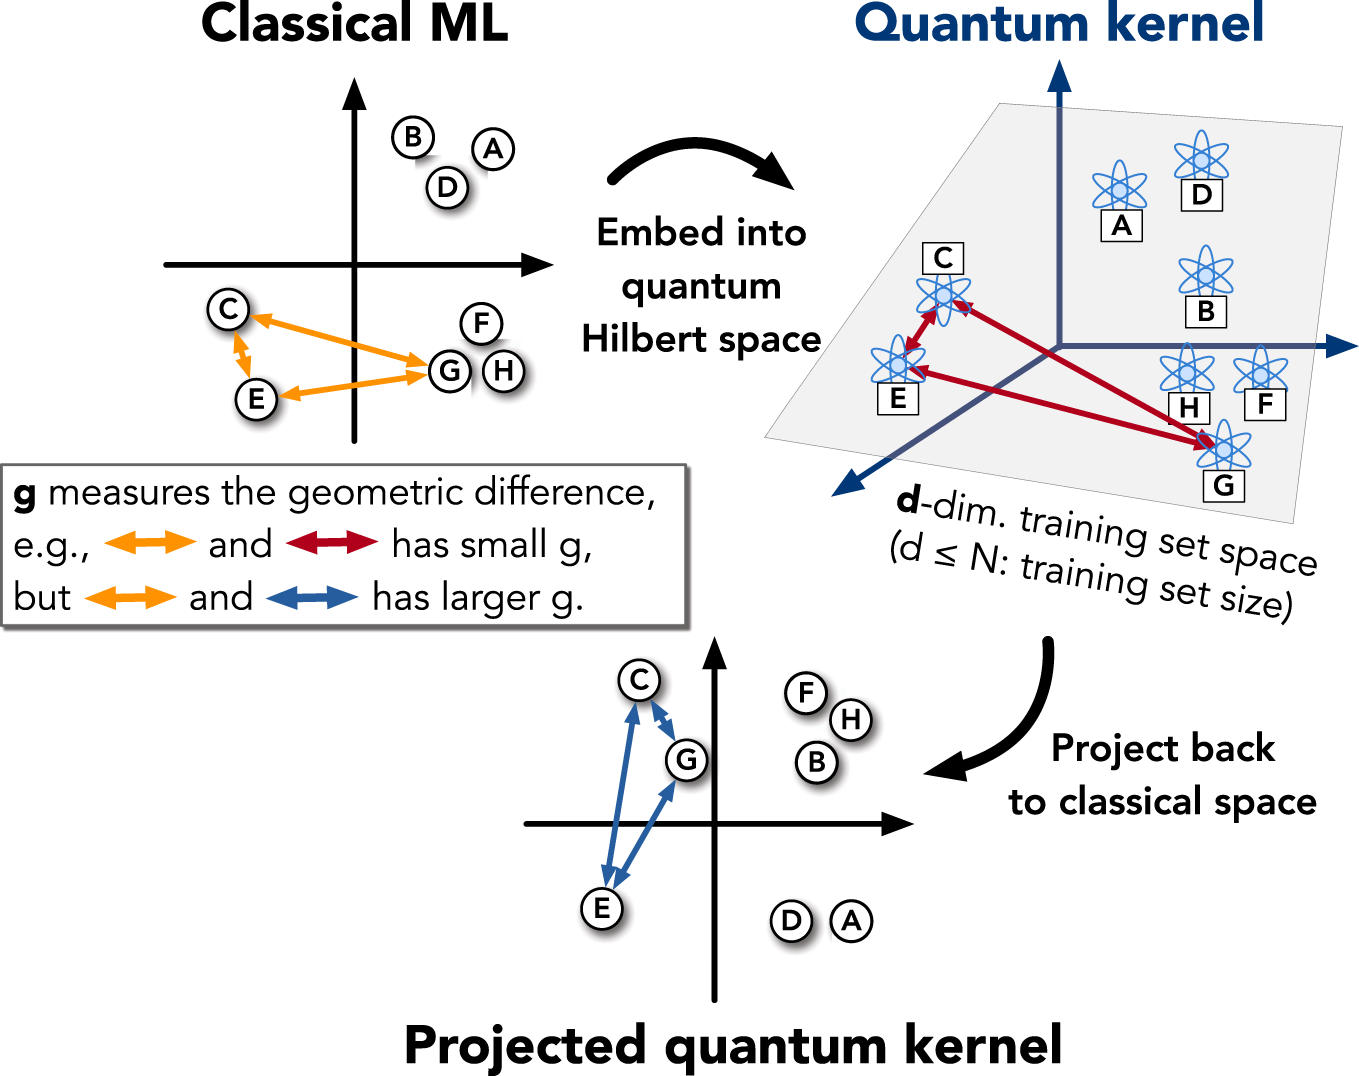
\includegraphics[width=0.7\textwidth]{Figures/Huang2021_Fig2.png}
  \caption{Geometría (función kernel) definida por modelos clásicos y cuánticos. Las letras
  representan datos y las flechas, la similitud entre ellos; la \textit{geometric difference}
  \(g\) mide cuánto difieren esas similitudes entre modelos, y \(d\) es la dimensión efectiva
  del conjunto de entrenamiento en el espacio de Hilbert. Reproducida de Huang et al. (2021),
  \textit{Nat. Commun.} 12, 2631, bajo licencia CC BY 4.0 (\protect\url{https://creativecommons.org/licenses/by/4.0/}).}
  \label{fig:huang_geometria}
\end{figure}

\textbf{Concentración exponencial del kernel cuántico.}
Un obstáculo para escalar de clasificadores cuánticos basados en producto interno
es el fenómeno de concentración, advertido por Huang et al. (``\textit{all inputs are too far apart}'')
y formalizado por Thanasilp et al. \cite{Thanasilp2024}. A medida que el número de qubits $n$
crece, las fidelidades cuánticas fuera de la diagonal
$|\langle\phi(\mathbf{x})|\phi(\mathbf{x}')\rangle|^2$ se concentran exponencialmente en $n$ alrededor de un valor fijo, que para el kernel de fidelidad
es cercano a cero. El kernel se acerca entonces a la matriz identidad, $K_Q \approx I$: todas las
muestras parecen casi ortogonales entre sí y se pierde la noción de vecindad.
Thanasilp et al. identifican cuatro fuentes de concentración: la expresividad del \textit{embedding},
las mediciones globales (como el proyector $|0\dots 0\rangle\langle 0\dots 0|$ con que se estima el kernel
de fidelidad), el entrelazamiento y el ruido. Los
resultados empíricos sobre la concentración observada en este proyecto se presentan en la sección de resultados.

% ---
% Subsección nueva en Docs/Technical_Report.tex
% Decisiones: D-033, H-038, H-039
% ---

\subsubsection{Dimensión efectiva}
\label{sec:dimension_efectiva}

Para caracterizar la expresividad y la estructura espectral de la matriz de kernel sin
depender de las etiquetas de clase, Huang et al. \cite{huang2021power} propusieron el concepto
de \textit{dimensión efectiva} $d(K)$. Esta métrica cuantifica cuántas direcciones
independientes u ortogonales explora el conjunto de datos en el espacio de Hilbert inducido
por el kernel.

Sea $K \in \mathbb{R}^{N \times N}$ una matriz de kernel normalizada a traza $N$
($\operatorname{Tr}(K) = N$). Sean $t_1 \ge t_2 \ge \dots \ge t_N \ge 0$ los autovalores
ordenados de forma decreciente de $K$. La dimensión efectiva se define como:
\begin{equation}
  d(K) = \sum_{k=1}^{N} \frac{1}{N - k + 1}\sum_{l=k}^{N} t_l.
  \label{eq:dim_efectiva}
\end{equation}
En la ecuación~\eqref{eq:dim_efectiva}, el término interior $\sum_{l=k}^{N} t_l$ representa
la suma de la cola espectral a partir del $k$-ésimo autovalor, y el denominador
la promedia entre las $N-k+1$ direcciones restantes.

% respaldo: «In the numerical experiment, we choose the following measure as the approximate dimension» (huang2021powerSupp, p. 12)
% La errata está igual en la versión publicada (S64) y en la de arXiv (F12), sección 6 B = Apéndice F.2.
\textbf{Nota sobre errata en la literatura:} La ecuación (S64) de la información suplementaria de Huang et al. \cite{huang2021power} (sección~6\,B) imprime el factor normalizador como $\frac{1}{N - k}$, formulación que incurre en una indeterminación por división entre cero en el último sumando ($k = N$). La corrección consiste en emplear el denominador $N - k + 1$. Con esta formulación, la métrica satisface las cotas que enuncian los autores:
\begin{equation}
  1 \le d(K) \le N.
  \label{eq:effective_dim_bounds}
\end{equation}
Los dos extremos se comprueban directamente:
\begin{itemize}
  \item \textbf{Cota inferior ($d = 1$):} Si todas las muestras mapean al mismo estado cuántico, la matriz de kernel tiene rango 1 ($t_1 = N$ y $t_l = 0$ para $l \ge 2$). La suma total colapsa a $d = \frac{1}{N} t_1 = \frac{N}{N} = 1$.
  \item \textbf{Cota superior ($d = N$):} Si todas las muestras mapean a estados mutuamente ortogonales en el espacio de Hilbert ($K = I$, autovalores $t_l = 1$ para todo $l$), la cola espectral para cada índice $k$ satisface $\sum_{l=k}^N 1 = N - k + 1$. Al cancelarse con el denominador, cada sumando vale idénticamente 1, resultando en $d = \sum_{k=1}^N 1 = N$.
\end{itemize}

Valores de $d$ cercanos a $N$ indican que cada lesión ocupa casi su propia dirección, como ocurre con un kernel concentrado; valores pequeños, que el kernel agrupa las lesiones en pocas direcciones.

% ---
% Reemplaza líneas 1803-1844 de Docs/Technical_Report.tex
% Decisiones: D-016, D-033
% ---

\subsubsection{Índice Davies-Bouldin}

El índice Davies-Bouldin (DB) \cite{davies1979cluster}
mide la calidad de la separación entre clusters en un
espacio de representación, combinando la dispersión
intra-clase con la separación inter-clase. Para el
problema de clasificación binaria (benigno / maligno),
las dos clases diagnósticas se definen como clusters
predeterminados ($C = 2$). El índice se define como:

\begin{equation}
  \text{DB} =
  \frac{1}{C}\sum_{i=1}^{C}
  \max_{j \neq i}
  \left\{
  \frac{s_i + s_j}{d(c_i, c_j)}
  \right\}
  \label{eq:davies_bouldin}
\end{equation}

\noindent donde $C = 2$ es el número de clases,
$s_i$ es la dispersión promedio de los puntos de la
clase $i$ respecto a su centroide $c_i$:

\begin{equation}
  s_i = \frac{1}{|C_i|}
  \sum_{\mathbf{z} \in C_i}
  \|\mathbf{z} - c_i\|_2
  \label{eq:dispersion}
\end{equation}

\noindent y $d(c_i, c_j) = \|c_i - c_j\|_2$ es la
distancia euclidiana entre los centroides de las clases
$i$ y $j$. Valores bajos del índice DB indican clusters
compactos y bien separados; el valor óptimo es 0.
Esta métrica es independiente del clasificador y puede
aplicarse directamente sobre el vector de embeddings
$\mathbf{e}(\mathbf{x}, \boldsymbol{\theta})$ de las
condiciones cuánticas o sobre los vectores transformados
de las condiciones clásicas. Al depender de distancias
euclidianas invariantes ante rotaciones ortogonales,
el índice DB genera el mismo valor para C1 y C2.

% ---
% Reemplaza líneas 1845-1883 de Docs/Technical_Report.tex
% Decisiones: D-016, D-033
% ---

\subsubsection{Razón multivariante de Fisher}

La razón de Fisher cuantifica la separabilidad lineal entre dos clases comparando la
distancia entre sus centroides frente a la dispersión intraclase. En el análisis univariado
clásico introducido por Fisher \cite{fisher1936use}, el coeficiente mide la separación a lo
largo de un único eje. Sin embargo, en un espacio de representación multivariado $\mathbb{R}^k$
(como el espacio de $k = 12$ dimensiones de los embeddings cuánticos o de las características
radiómicas), la formulación unidimensional promediada coordenada por coordenada ignora las
covarianzas entre variables y adolece de una limitación geométrica: no es invariante
ante transformaciones de rotación.

Para garantizar consistencia metodológica, en este trabajo se adopta la
\textit{razón multivariante de Fisher} (distancia de Mahalanobis al cuadrado entre medias de
clase con la matriz de covarianza combinada):
\begin{equation}
  J = \Delta\boldsymbol{\mu}^\top S_W^{-1} \Delta\boldsymbol{\mu},
  \label{eq:fisher_multivariate}
\end{equation}
donde $\Delta\boldsymbol{\mu} = \boldsymbol{\mu}_1 - \boldsymbol{\mu}_0$ denota el vector de
diferencia entre los centroides de las clases maligna y benigna en $\mathbb{R}^k$, y $S_W$ es
la matriz de dispersión intraclase combinada (\textit{pooled within-class covariance}):
\begin{equation}
  S_W = \frac{1}{N - 2} \left[ \sum_{i \in \mathcal{C}_0} (\mathbf{e}_i - \boldsymbol{\mu}_0)(\mathbf{e}_i - \boldsymbol{\mu}_0)^\top + \sum_{j \in \mathcal{C}_1} (\mathbf{e}_j - \boldsymbol{\mu}_1)(\mathbf{e}_j - \boldsymbol{\mu}_1)^\top \right].
  \label{eq:pooled_covariance}
\end{equation}
La formulación matricial de la ecuación~\eqref{eq:fisher_multivariate} posee una propiedad
algebraica relevante: es invariante ante cualquier transformación afín
invertible del espacio de características, $\mathbf{e} \mapsto A\mathbf{e} + \mathbf{b}$,
con $A \in \mathbb{R}^{k \times k}$ y $\det(A) \neq 0$:
\begin{align}
  J(A\mathbf{e} + \mathbf{b}) &= (A\Delta\boldsymbol{\mu})^\top (A S_W A^\top)^{-1} (A\Delta\boldsymbol{\mu}) \nonumber \\
  &= \Delta\boldsymbol{\mu}^\top A^\top (A^\top)^{-1} S_W^{-1} A^{-1} A \Delta\boldsymbol{\mu} \nonumber \\
  &= \Delta\boldsymbol{\mu}^\top S_W^{-1} \Delta\boldsymbol{\mu} = J(\mathbf{e}).
  \label{eq:fisher_affine_invariance}
\end{align}
Esta invariancia afín es necesaria para el diseño experimental del proyecto. La condición
C2 aplica una transformación por Componentes Principales completa sin reducción de dimensión
($k \to k$). Dicha proyección es una traslación seguida de una rotación ($A \in \mathrm{O}(k)$),
por lo que, bajo la formulación multivariante, se cumple necesariamente que
$J(\text{C1}) = J(\text{C2})$ por construcción.

% ---
% Reemplaza líneas 1884-1906 de Docs/Technical_Report.tex
% Decisiones: D-033
% ---

\subsubsection{Visualización \textit{t-SNE}}

El algoritmo \textit{t-Distributed Stochastic Neighbor
Embedding} (t-SNE) \cite{vandermaaten2008tsne} proyecta
vectores de alta dimensionalidad a un espacio de dos
dimensiones preservando la estructura de vecindad local.
Se utiliza como herramienta de visualización cualitativa
de la separabilidad de clases en el espacio de embeddings:
si la proyección t-SNE muestra clusters compactos y bien
separados por clase, el espacio de representación tiene
estructura discriminativa.

Como complemento visual de las métricas de separabilidad del espacio de embeddings
(DB, Fisher multivariante y KTA lineal), t-SNE se emplea como herramienta de exploración cualitativa.
Para garantizar reproducibilidad, la proyección bidimensional se genera fijando
perplejidad 30, inicialización determinista basada en las dos primeras componentes principales
(PCA) y semilla aleatoria 42 (\texttt{sklearn.manifold.TSNE}). Se utiliza con fines
de soporte visual y no como criterio numérico de decisión.

% ---
% Reemplaza líneas 1907-1967 de Docs/Technical_Report.tex
% Decisiones: D-018, D-036
% ---

\subsubsection{Métricas de clasificación}

El desempeño del clasificador MLP sobre cada condición experimental se evalúa a partir de
las predicciones de probabilidad de malignidad $\hat{y} \in [0, 1]$ generadas por la función
sigmoide de salida. Para las métricas dependientes de umbral, se adopta el umbral de decisión
operativo estándar de 0.5 ($\hat{y} \geq 0.5 \implies \text{maligno}$):

\textbf{Exactitud (\textit{Accuracy}):}
\begin{equation}
  \text{Acc} =
  \frac{TP + TN}{TP + TN + FP + FN}
  \label{eq:accuracy}
\end{equation}

\textbf{Precisión (\textit{Precision}):}
\begin{equation}
  \text{Prec} =
  \frac{TP}{TP + FP}
  \label{eq:precision}
\end{equation}

\textbf{Exhaustividad (\textit{Recall}):}
\begin{equation}
  \text{Rec} =
  \frac{TP}{TP + FN}
  \label{eq:recall}
\end{equation}

\textbf{F1-Score:}
\begin{equation}
  F_1 =
  \frac{2 \cdot \text{Prec} \cdot \text{Rec}}
  {\text{Prec} + \text{Rec}}
  \label{eq:f1}
\end{equation}

\textbf{Área bajo la curva ROC (AUC-ROC):}
\begin{equation}
  \text{AUC} =
  \int_0^1 \text{TPR}(t)\,d\,\text{FPR}(t)
  \label{eq:auc_roc}
\end{equation}

\noindent donde $TP$, $TN$, $FP$ y $FN$ son los
verdaderos positivos, verdaderos negativos, falsos
positivos y falsos negativos respectivamente;
$\text{TPR}(t) = TP/(TP+FN)$ es la tasa de verdaderos
positivos y $\text{FPR}(t) = FP/(FP+TN)$ es la tasa
de falsos positivos, ambas evaluadas al umbral de
decisión $t$.

El \textbf{Área bajo la curva ROC (AUC-ROC)}, formalizada en la ecuación~\eqref{eq:auc_roc},
constituye la métrica principal de comparación técnica entre condiciones. Al integrar la
tasa de verdaderos positivos en función de la tasa de falsos positivos sobre la totalidad de
los umbrales posibles $t \in [0, 1]$, el AUC-ROC cuantifica la capacidad discriminativa intrínseca
del modelo con independencia del umbral operativo y de forma robusta frente al desbalance
de clases del CBIS-DDSM.

El protocolo de validación evalúa todas las métricas mediante validación cruzada de 5 \textit{folds}
estratificada por clase y agrupada por paciente sobre el conjunto de entrenamiento, así
como mediante una evaluación final sobre el conjunto de prueba oficial, que se usa una sola vez por modelo, reportando
intervalos de confianza al 95\,\% derivados de 2\,000 remuestreos \textit{bootstrap} pareados por
paciente.

% ---
% Reemplaza líneas 1968-2007 de Docs/Technical_Report.tex
% Decisiones: D-016, D-039, H-049
% ---

\subsubsection{Análisis de correlación separabilidad--clasificación}

Para dar cumplimiento al objetivo específico OE-5, se evalúa si la jerarquía de separabilidad
geométrica observada en el espacio de representación predice el desempeño predictivo alcanzado
por el clasificador MLP. Para cuantificar la concordancia monótona entre los ordenamientos de las
cinco condiciones experimentales (C1 a C5), se calcula el coeficiente de correlación de rangos
de Spearman $\rho_s$.

La fórmula $1-6\sum d_i^2/(n(n^2-1))$ solo vale sin empates. En el diseño metodológico del presente trabajo,
las condiciones C1 y C2 arrojan idénticos valores de separabilidad por construcción matemática
(invariancia rotacional de Davies-Bouldin, Fisher multivariante y KTA lineal). Al asignarse
rangos promedio a las condiciones empatadas, las sumas de cuadrados de los rangos disminuyen
respecto al caso de rangos discretos enteros, lo que invalida la fórmula de diferencias
cuadráticas. La definición de $\rho_s$, adoptada en este trabajo, corresponde a
la \textit{correlación de Pearson evaluada sobre los rangos promedio}:
\begin{equation}
  \rho_s = \frac{\sum_{i=1}^{n} (R_i - \bar{R})(S_i - \bar{S})}{\sqrt{\sum_{i=1}^{n} (R_i - \bar{R})^2 \sum_{i=1}^{n} (S_i - \bar{S})^2}},
  \label{eq:spearman}
\end{equation}
donde $R_i$ representa el rango asignado a la condición $i$ según la métrica de separabilidad, $S_i$
denota el rango de la condición según el AUC-ROC de clasificación, y $\bar{R} = \bar{S} = \frac{n+1}{2} = 3$
es la media teórica de los rangos para $n = 5$ condiciones. A las condiciones C1 y C2 se les asigna
el rango medio compartido correspondiente a las posiciones que ocupan conjuntamente.

Debido al tamaño reducido del conjunto de condiciones ($n = 5$), el espacio muestral de posibles
permutaciones consta de exactamente $5! = 120$ órdenes posibles, todos equiprobables bajo la hipótesis
nula de ordenamiento aleatorio. En este régimen de muestra pequeña, las aproximaciones asintóticas
estándar (como la distribución $t$ de Student) carecen de validez, y la distribución nula exacta es
discreta:
\begin{itemize}
  \item sin empates, solo $\rho_s=\pm1$ llega a $p<0.05$ bilateral, $p = 2/120 \approx 0.017$, y una sola inversión de vecinos da $\rho_s = 0.9$ con $p = 10/120 \approx 0.083$;
  \item con el empate C1 = C2, el máximo es $\rho_s=\sqrt{19/20}\approx0.975$, alcanzado por 2 de los 120 órdenes, con $p$ bilateral $= 4/120 \approx 0.033$.
\end{itemize}
Por esta razón, el coeficiente de Spearman entre separabilidad y clasificación se reporta con
carácter descriptivo por subproblema (masas y calcificaciones), complementado con su
distribución nula exacta tabulada, evaluando cualitativamente si las
tres condiciones clásicas (C1, C2, C3) se posicionan sistemáticamente por encima de las dos
cuánticas (C4, C5) tanto en separabilidad como en desempeño clasificatorio.

% ---
% Subsección nueva en TT2 (2026-10-18), al final del Marco Teórico para no renumerar lo aprobado.
% Reúne los métodos clásicos y de kernel que usan la Metodología y los Resultados: la radiómica (M3),
% PCA y Kernel PCA (C2 y C3, D-016, D-027), la SVM y el QSVM (X4, D-038) y el kernel proyectado (X6).
% ---

\subsection{Representaciones clásicas y modelos de kernel}
\label{sec:representaciones_clasicas}

Las secciones anteriores describen la parte cuántica del sistema. Esta reúne los métodos clásicos que la rodean: la extracción radiómica, que produce el vector de características de cada lesión; las dos transformaciones clásicas con las que se comparan las cuánticas, el análisis de componentes principales y su versión con kernel, y los modelos de kernel que se usan en los experimentos complementarios.

% ---
% Subsubsección 3.5.1 (nueva, 2026-10-18). Base teórica del Módulo 3 (D-008, D-023).
% La ecuación de discretización es la del manual IBSI (Zwanenburg2020IBSI, p. 23).
% Cada atribución lleva su respaldo verificable con Code/tools/verificar_citas_fichas.py.
% ---

\subsubsection{Características radiómicas}
\label{sec:radiomica}

% respaldo: «These advances have facilitated the development of processes for high-throughput extraction of quantitative features that result in the conversion of images into mineable data and the subsequent analysis of these data for decision support; this practice is termed radiomics.» (Gillies2016Radiomics, p. 1)
La radiómica es la extracción, a gran escala, de características cuantitativas de las imágenes médicas, que convierte las imágenes en datos analizables y permite usarlos como apoyo a la decisión \cite{Gillies2016Radiomics}. En este trabajo, cada lesión se describe con 67 características calculadas con PyRadiomics \cite{vanGriethuysen2017} sobre la región de interés, agrupadas en cuatro familias: primer orden, forma, matriz de co-ocurrencia de niveles de gris (GLCM) y matriz de longitudes de secuencia (GLRLM). Su configuración se detalla en la sección~\ref{sec:modulo3}.

\textbf{Discretización de intensidades}

% respaldo: «In the fixed bin number method, intensities Xgl are discretised to a fixed number of Ng bins.» (Zwanenburg2020IBSI, p. 23)
Las familias de textura no trabajan con las intensidades originales, sino con niveles de gris discretos. Con el método de número fijo de niveles que define el manual de la \textit{Image Biomarker Standardisation Initiative} (IBSI), la intensidad $X_k$ de cada píxel de la región se lleva a uno de $N_g$ niveles \cite{Zwanenburg2020IBSI}:
\begin{equation}
  X_{d,k} =
  \begin{cases}
    \left\lfloor N_g \dfrac{X_k - X_{\min}}{X_{\max} - X_{\min}} \right\rfloor + 1, & X_k < X_{\max},\\[8pt]
    N_g, & X_k = X_{\max},
  \end{cases}
  \label{eq:discretizacion}
\end{equation}
donde $X_{\min}$ y $X_{\max}$ son la menor y la mayor intensidad dentro de la región. En este trabajo $N_g = 32$. Como el rango se toma de cada lesión, el método no depende de la escala absoluta de las intensidades, que en el CBIS-DDSM no está calibrada.

\textbf{Primer orden y forma}

Las características de primer orden son estadísticas de la distribución de intensidades dentro de la región, sin información espacial: la media, los percentiles, la asimetría o la entropía,
\begin{equation}
  H = -\sum_{i=1}^{N_g} p(i)\,\log_2 p(i),
  \label{eq:entropia_radiomica}
\end{equation}
donde $p(i)$ es la fracción de píxeles de la región con nivel de gris $i$. Las de forma describen la geometría del contorno de la máscara: área, perímetro, ejes mayor y menor, elongación. Como los DICOM del CBIS-DDSM no traen el espaciado de píxel, las medidas de forma quedan en píxeles.

\textbf{Matriz de co-ocurrencia (GLCM)}

% respaldo: «The grey level co-occurrence matrix (GLCM) is a matrix that expresses how combinations of discretised intensities (grey levels) of neighbouring pixels, or voxels in a 3D volume, are distributed along one of the image directions.» (Zwanenburg2020IBSI, p. 69)
La GLCM describe cómo se combinan los niveles de gris de píxeles vecinos a lo largo de una dirección de la imagen \cite{Zwanenburg2020IBSI}. Para una distancia $\delta$ y una dirección $\theta$, su elemento $P(i,j \mid \delta,\theta)$ cuenta cuántos pares de píxeles separados por $\delta$ en la dirección $\theta$ tienen los niveles $i$ y $j$. Normalizada, $p(i,j) = P(i,j)/\sum_{i,j}P(i,j)$, es una distribución conjunta de la que se derivan las características; por ejemplo, el contraste,
\begin{equation}
  \text{Contraste} = \sum_{i=1}^{N_g}\sum_{j=1}^{N_g} (i-j)^2\, p(i,j),
  \label{eq:glcm_contraste}
\end{equation}
que crece cuando los vecinos tienen niveles muy distintos. En este trabajo, $\delta = 1$ y las características se promedian sobre las cuatro direcciones del plano.

\textbf{Matriz de longitudes de secuencia (GLRLM)}

% respaldo: «whereas GLCM assesses co-occurrence of grey levels within neighbouring pixels or voxels, GLRLM assesses run lengths. A run length is defined as the length of a consecutive sequence of pixels or voxels with the same grey level along direction m, which was previously defined in Section 3.6.» (Zwanenburg2020IBSI, p. 92)
La GLRLM evalúa secuencias: una secuencia es un tramo de píxeles consecutivos con el mismo nivel de gris a lo largo de una dirección \cite{Zwanenburg2020IBSI}. Su elemento $R(i,j \mid \theta)$ cuenta cuántas secuencias de nivel $i$ y longitud $j$ hay en la dirección $\theta$. Con $N_r$ el número total de secuencias, el énfasis en secuencias cortas,
\begin{equation}
  \text{SRE} = \frac{1}{N_r}\sum_{i=1}^{N_g}\sum_{j} \frac{R(i,j)}{j^2},
  \label{eq:glrlm_sre}
\end{equation}
es alto en texturas finas, donde el nivel de gris cambia de un píxel al siguiente, y bajo en regiones homogéneas.

% ---
% Subsubsección 3.5.2 (nueva, 2026-10-18). Condición C2 (D-016: control nulo).
% Implementación: sklearn.decomposition.PCA(n_components=12), ajustada solo en train (5a_Embeddings).
% Que la rotación completa conserva las distancias se comprobó numéricamente: diferencia máxima
% de 6e-15 entre distancias euclidianas antes y después del PCA con 12 de 12 componentes.
% ---

\subsubsection{Análisis de componentes principales (PCA)}
\label{sec:pca}

El análisis de componentes principales (PCA) busca las direcciones de máxima varianza de los datos \cite{goodfellow2016deep}. Sea $\boldsymbol{\mu}$ la media de los vectores de entrenamiento y $\tilde{X}$ la matriz de entrenamiento centrada, con una lesión por fila. La matriz de covarianza se descompone como
\begin{equation}
  \Sigma = \frac{1}{n-1}\,\tilde{X}^{\top}\tilde{X} = V \Lambda V^{\top},
  \label{eq:pca_covarianza}
\end{equation}
donde las columnas de $V$ son los vectores propios ortonormales y $\Lambda$ es la matriz diagonal de varianzas, en orden decreciente. La representación de una lesión $\mathbf{x}$ es su proyección sobre esas direcciones:
\begin{equation}
  \mathbf{z} = V^{\top}(\mathbf{x} - \boldsymbol{\mu}).
  \label{eq:pca_proyeccion}
\end{equation}

Cuando se conservan menos componentes que variables, PCA reduce la dimensión. En la condición C2 se conservan las $k = 12$, de modo que $V$ es una matriz ortogonal de $12 \times 12$ y la transformación es una traslación seguida de una rotación. Una rotación conserva las distancias y los productos internos de los datos centrados:
\begin{equation}
  \lVert \mathbf{z} - \mathbf{z}' \rVert = \lVert V^{\top}(\mathbf{x} - \mathbf{x}') \rVert = \lVert \mathbf{x} - \mathbf{x}' \rVert.
  \label{eq:pca_isometria}
\end{equation}
Por eso C2 es un control nulo: toda métrica de separabilidad que dependa solo de distancias o de productos internos centrados da el mismo valor en C1 y en C2. Si una métrica distinguiera ambas condiciones, la diferencia vendría de la implementación y no de la geometría. El clasificador, en cambio, no es invariante ante rotaciones, porque estandariza cada coordenada por separado, y puede dar resultados ligeramente distintos en C1 y C2.

% ---
% Subsubsección 3.5.3 (nueva, 2026-10-18). Condición C3 (D-027: γ por la heurística de la mediana).
% Implementación: sklearn.decomposition.KernelPCA(n_components=12, kernel='rbf', gamma=γ), ajustada
% solo en train (5a_Embeddings). La normalización de la ec. de proyección es la de scikit-learn: sobre
% los puntos de entrenamiento, la componente ℓ vale sqrt(μ_ℓ) veces el vector propio.
% ---

\subsubsection{Análisis de componentes principales con kernel (Kernel PCA)}
\label{sec:kernel_pca}

El Kernel PCA aplica el análisis de componentes principales en el espacio de características de un kernel, sin calcular ese espacio de forma explícita \cite{Scholkopf1998KPCA}. Es la contraparte clásica no lineal de un \textit{feature map}: como el kernel cuántico de fidelidad (ecuación~\eqref{eq:quantum_kernel}), un kernel $k(\mathbf{x},\mathbf{x}')$ define implícitamente un mapa $\phi$ con $k(\mathbf{x},\mathbf{x}') = \langle \phi(\mathbf{x}), \phi(\mathbf{x}') \rangle$, y todo el cálculo se hace a través de $k$.

Con los $n$ vectores de entrenamiento se forma la matriz $K_{ij} = k(\mathbf{x}_i, \mathbf{x}_j)$ y se centra en el espacio de características:
\begin{equation}
  \tilde{K} = K - \mathbf{1}_n K - K \mathbf{1}_n + \mathbf{1}_n K \mathbf{1}_n,
  \label{eq:kpca_centrado}
\end{equation}
donde $\mathbf{1}_n$ es la matriz de $n \times n$ con todas sus entradas iguales a $1/n$. Si $\mu_\ell$ y $\mathbf{a}^{\ell}$ son los valores y vectores propios unitarios de $\tilde{K}$, la componente $\ell$ de una lesión $\mathbf{x}$ es
\begin{equation}
  z_\ell(\mathbf{x}) = \frac{1}{\sqrt{\mu_\ell}} \sum_{i=1}^{n} a^{\ell}_i\, \tilde{k}(\mathbf{x}_i, \mathbf{x}),
  \label{eq:kpca_proyeccion}
\end{equation}
donde $\tilde{k}$ es el kernel centrado con las medias de entrenamiento. Sobre los puntos de entrenamiento, $z_\ell(\mathbf{x}_j) = \sqrt{\mu_\ell}\, a^{\ell}_j$.

En la condición C3 se usa el kernel gaussiano (RBF),
\begin{equation}
  k(\mathbf{x}, \mathbf{x}') = \exp\!\left(-\gamma \lVert \mathbf{x} - \mathbf{x}' \rVert^2\right),
  \qquad
  \gamma = \frac{1}{2\,\operatorname{med}_{i<j}\lVert \mathbf{x}_i - \mathbf{x}_j \rVert^2},
  \label{eq:rbf_mediana}
\end{equation}
con $\gamma$ fijado por la heurística de la mediana sobre las distancias de entrenamiento, y se conservan 12 componentes, la misma dimensión que las demás condiciones. A diferencia de C2, C3 es no lineal: deforma la geometría de los datos, como lo hacen los mapas cuánticos, pero con un kernel clásico. Por eso es la comparación clásica más directa para C4 y C5. Los kernels gaussianos forman también parte de la batería de kernels clásicos de referencia con la que se calcula la \textit{geometric difference} (sección~\ref{sec:metricas}).

% ---
% Subsubsección 3.5.4 (nueva, 2026-10-18), breve por decisión del autor. Se usa en X4 y X6 (D-038).
% Implementación: sklearn.svm.SVC(kernel='precomputed', C=1, class_weight='balanced').
% ---

\subsubsection{Máquina de vectores de soporte (SVM)}
\label{sec:svm}

La máquina de vectores de soporte (SVM) separa dos clases con el hiperplano de margen máximo, admitiendo errores con una penalización $C$ \cite{CortesVapnik1995}. En su forma dual, la función de decisión solo depende de los datos a través de un kernel:
\begin{equation}
  f(\mathbf{x}) = \sum_{i=1}^{n} \alpha_i\, y_i\, k(\mathbf{x}_i, \mathbf{x}) + b,
  \qquad 0 \le \alpha_i \le C_{y_i},
  \label{eq:svm_dual}
\end{equation}
con $y_i \in \{-1, +1\}$. Los $\mathbf{x}_i$ con $\alpha_i > 0$ son los vectores de soporte. Como el modelo solo necesita la matriz de kernel, puede entrenarse con cualquier kernel semidefinido positivo, clásico o cuántico, sin cambiar el algoritmo. En los experimentos complementarios se usa con $C = 1$ y con $C_{y}$ ponderado de forma inversa a la frecuencia de cada clase.

% ---
% Subsubsección 3.5.5 (nueva, 2026-10-18), breve por decisión del autor. Experimento X4 (D-038, H-044).
% Implementación: kernel de fidelidad exacto por vector de estado (sin ansatz) y SVC precomputada.
% Cada atribución lleva su respaldo verificable con Code/tools/verificar_citas_fichas.py.
% ---

\subsubsection{Máquina de vectores de soporte cuántica (QSVM)}
\label{sec:qsvm}

% respaldo: «In the second, a quantum kernel estimator, we estimate the kernel function and optimize the classifier directly.» (havlicek2019supervised, p. 1)
Una QSVM es una SVM cuyo kernel se estima con un circuito cuántico \cite{havlicek2019supervised}: en la ecuación~\eqref{eq:svm_dual} se usa el kernel de fidelidad $k(\mathbf{x},\mathbf{x}') = |\langle \phi(\mathbf{x}) | \phi(\mathbf{x}') \rangle|^2$ de la ecuación~\eqref{eq:quantum_kernel}. El computador cuántico solo calcula la matriz de kernel; el entrenamiento de la SVM es clásico. En un procesador real, cada entrada se estima midiendo el circuito $U^{\dagger}(\mathbf{x}')\,U(\mathbf{x})$ sobre $|0\rangle^{\otimes n}$ y contando la fracción de veces que el resultado es la cadena de ceros, por lo que su precisión depende del número de mediciones. En simulación de vector de estado se calcula de forma exacta.

En este trabajo, la QSVM se usa en un experimento complementario, con los mapas de C4 y C5 y el mismo protocolo que una SVM con kernel RBF (sección~\ref{sec:qsvm_ventaja}). Su interés es metodológico: como el kernel de fidelidad usa solo el \textit{feature map}, sin \textit{ansatz} ni medición de $\langle Z_i \rangle$, permite separar lo que la codificación cuántica conserva de lo que se pierde al leer los valores esperados.

% ---
% Subsubsección 3.5.6 (nueva, 2026-10-18). Experimento X6 (D-038, H-047, H-048).
% La identidad de la ec. eq:kpq_pauli se comprobó numéricamente con Qiskit (estados aleatorios de 3
% qubits, partial_trace frente a valores esperados de Pauli): diferencia de 1e-16.
% Implementación en X6: valores esperados <X_k>, <Y_k>, <Z_k> de los 12 qubits del ZZFeatureMap con
% c = 1 y kernel gaussiano sobre ellos, con cinco anchos de banda.
% Cada atribución lleva su respaldo verificable con Code/tools/verificar_citas_fichas.py.
% ---

\subsubsection{Kernel cuántico proyectado}
\label{sec:kernel_proyectado}

% respaldo: «To circumvent this setback, we propose a family of projected quantum kernels as a solution. These kernels work by projecting the quantum states to an approximate classical representation, e.g., using reduced physical observables or classical shadows25,27,42–44.» (huang2021power, p. 6)
El kernel de fidelidad compara estados en el espacio de Hilbert completo, de dimensión $2^n$, donde, como se vio en la sección~\ref{sec:limites_ventaja}, las entradas tienden a quedar demasiado lejos entre sí. Huang et al. propusieron los kernels cuánticos proyectados, que primero proyectan cada estado a una representación clásica aproximada, por ejemplo mediante observables reducidos, y después comparan esas representaciones \cite{huang2021power}.

% respaldo: «One of the simplest forms of projected quantum kernel is to measure the one-particle reduced density matrix (1-RDM) on all qubits for the encoded state» (huang2021power, p. 6)
La forma más simple usa la matriz de densidad reducida de cada qubit \cite{huang2021power}. Si $\rho(\mathbf{x}) = |\phi(\mathbf{x})\rangle\langle\phi(\mathbf{x})|$ es el estado codificado y $\rho_k(\mathbf{x}) = \operatorname{Tr}_{j \neq k}[\rho(\mathbf{x})]$ el del qubit $k$, que se obtiene trazando los demás, el kernel es
\begin{equation}
  k^{\mathrm{PQ}}(\mathbf{x}, \mathbf{x}') = \exp\!\left(-\gamma \sum_{k=1}^{n} \bigl\lVert \rho_k(\mathbf{x}) - \rho_k(\mathbf{x}') \bigr\rVert_F^2\right).
  \label{eq:kpq}
\end{equation}

Esta expresión tiene una lectura directa en términos de mediciones. El estado de un qubit se escribe como $\rho_k = \tfrac{1}{2}\bigl(I + \sum_{P} \langle P_k \rangle\, P\bigr)$, con $P \in \{X, Y, Z\}$, y como $\operatorname{Tr}(PQ) = 2\,\delta_{PQ}$ para las matrices de Pauli,
\begin{equation}
  \bigl\lVert \rho_k(\mathbf{x}) - \rho_k(\mathbf{x}') \bigr\rVert_F^2 = \frac{1}{2} \sum_{P \in \{X,Y,Z\}} \bigl(\langle P_k \rangle_{\mathbf{x}} - \langle P_k \rangle_{\mathbf{x}'}\bigr)^2 .
  \label{eq:kpq_pauli}
\end{equation}
El kernel proyectado es, por tanto, un kernel gaussiano con parámetro $\gamma/2$ sobre el vector de $3n$ valores esperados $\langle X_k \rangle$, $\langle Y_k \rangle$, $\langle Z_k \rangle$ de cada qubit. Se parece al \textit{quantum embedding} de la sección~\ref{sec:quantum_embedding}, con dos diferencias: aquí se leen los tres ejes de cada qubit, y se leen directamente sobre el estado del \textit{feature map}, sin \textit{ansatz}. Su parámetro $\gamma$ es un ancho de banda que se elige como en un kernel clásico.

% Añadido el 2026-10-23 (D-043, D-044): resume las tres formas de usar el estado del feature map que
% aparecen en el reporte. Las cifras de cada una están en la tabla tab:tres_lecturas de la sección 6.4.
Con este kernel, el reporte usa el estado de un mismo \textit{feature map} de tres maneras, que
difieren en qué se obtiene del estado y en cómo se comparan dos lesiones (tabla~\ref{tab:lecturas_estado}).
La distinción importa porque las tres pueden llevar a conclusiones distintas sobre la misma codificación.

\begin{table}[htbp]
\centering
\small
\caption{Tres formas de leer el estado $|\phi(\mathbf{x})\rangle$ de un mismo \textit{feature map}.}
\label{tab:lecturas_estado}
\begin{adjustbox}{max width=\linewidth}
\begin{tabular}{p{0.2\linewidth} p{0.25\linewidth} p{0.25\linewidth} p{0.25\linewidth}}
\toprule
 & \textbf{Valores esperados $\langle Z_i\rangle$} & \textbf{Kernel de fidelidad} & \textbf{Kernel proyectado} \\
\midrule
Circuito & \textit{Feature map} seguido del \textit{ansatz} $V(\boldsymbol\theta)$ & \textit{Feature map} & \textit{Feature map} \\
Qué se obtiene & $\langle Z_i\rangle$ de cada qubit tras el \textit{ansatz} & El solapamiento $|\langle\phi(\mathbf{x})|\phi(\mathbf{x}')\rangle|^2$ entre los estados completos & $\langle X_k\rangle$, $\langle Y_k\rangle$ y $\langle Z_k\rangle$ de cada qubit \\
Resultado & Un vector de $n$ valores por lesión & Un valor por par de lesiones & Un vector de $3n$ valores por lesión, comparado con un kernel gaussiano \\
Escala de la comparación & Local: un eje por qubit & Global: las $2^n$ amplitudes & Local: los tres ejes de cada qubit \\
Depende de $\boldsymbol\theta$ & Sí & No: $V(\boldsymbol\theta)$ se cancela & No: no hay \textit{ansatz} \\
Clasificador & Perceptrón multicapa & SVM (QSVM) & SVM \\
Medición en un procesador & Una base ($Z$) para todos los qubits & Un circuito \textit{compute-uncompute} por par de lesiones & Tres bases ($X$, $Y$, $Z$) \\
Dónde se usa & C4 y C5 (M5 y M7) & M6, X4 y X6 & X6 y X11 \\
\bottomrule
\end{tabular}
\end{adjustbox}
\end{table}

% respaldo: «In numerical experiments, we find that the classical projection increases rather than decreases the geometric difference with classical ML models.» (huang2021power, p. 6)
En los experimentos numéricos de Huang et al., esta proyección aumentó, en lugar de reducir, la \textit{geometric difference} con los modelos clásicos \cite{huang2021power}. En este trabajo se evalúa en un experimento complementario, sobre los estados del ZZFeatureMap con el factor de escala del diseño (sección~\ref{sec:qsvm_ventaja}).


% Bibliografía para 3_Marco_Teorico (solo claves citadas: 15)
\begin{thebibliography}{99}
\bibitem{Cortes2012}
    Cortes, C., Mohri, M., \& Rostamizadeh, A. (2012).
    Algorithms for learning kernels based on centered alignment.
    \textit{Journal of Machine Learning Research}, 13(28), 795--828.
    \url{https://jmlr.org/papers/v13/cortes12a.html}

\bibitem{Thanasilp2024}
    Thanasilp, S., Wang, S., Cerezo, M., \& Holmes, Z. (2024).
    Exponential concentration in quantum kernel methods.
    \textit{Nature Communications}, 15(1), 5200.
    \url{https://doi.org/10.1038/s41467-024-49287-w}

\bibitem{cerezo2021variational}
    Cerezo, M., Arrasmith, A., Babbush, R., Benjamin, S. C., Endo, S., Fujii, K., McClean, J. R., Mitarai, K., Yuan, X., Cincio, L., \& Coles, P. J. (2021). Variational quantum algorithms. \textit{Nature Reviews Physics}, 3, 625--644. \url{https://doi.org/10.1038/s42254-021-00348-9}

  % --- Referencia 32: Quantum Circuit Learning ---

\bibitem{cristianini2002kernel}
    Cristianini, N., Shawe-Taylor, J., Elisseeff, A., \& Kandola, J. (2002). On kernel-target alignment.
    In \textit{Advances in Neural Information Processing Systems (NeurIPS)}, 14.
    \url{https://proceedings.neurips.cc/paper/2001/hash/1f71e393b3809197ed66df836fe833e5-Abstract.html}

  % --- Referencia 37: Davies-Bouldin Cluster Separation Measure ---

\bibitem{davies1979cluster}
    Davies, D. L., \& Bouldin, D. W. (1979). A cluster separation measure.
    \textit{IEEE Transactions on Pattern Analysis and Machine Intelligence}, 1(2), 224--227.
    \url{https://doi.org/10.1109/TPAMI.1979.4766909}

  % --- Referencia 38: Fisher’s Linear Discriminant ---

\bibitem{fisher1936use}
    Fisher, R. A. (1936). The use of multiple measurements in taxonomic problems.
    \textit{Annals of Eugenics}, 7(2), 179--188.
    \url{https://doi.org/10.1111/j.1469-1809.1936.tb02137.x}

  % --- Referencia 39: t-SNE Data Visualization ---

\bibitem{goodfellow2016deep}
    Goodfellow, I., Bengio, Y., \& Courville, A. (2016). \textit{Deep Learning}. MIT Press.
    \url{https://www.deeplearningbook.org}

  % --- Referencia 36: Kernel-Target Alignment ---

\bibitem{havlicek2019supervised}
    Havl{\'{i}}{\v{c}}ek, V., C{\'{o}}rcoles, A. D., Temme, K., Harrow, A. W., Kandala, A., Chow, J. M., \& Gambetta, J. M. (2019). Supervised learning with quantum-enhanced feature spaces.
    \textit{Nature}, 567, 209--212.
    \url{https://doi.org/10.1038/s41586-019-0980-2}

  % --- Referencia 43: Power of Data in Quantum Machine Learning ---

\bibitem{huang2021power}
    Huang, H.-Y., Broughton, M., Mohseni, M., Babbush, R., Boixo, S., Neven, H., \& McClean, J. R. (2021). Power of data in quantum machine learning.
    \textit{Nature Communications}, 12, 2631.
    \url{https://doi.org/10.1038/s41467-021-22539-9}

  % --- Referencia 44: Realization of Contrast Limited Adaptive Histogram Equalization ---

\bibitem{ibmquantum2024docs}
    IBM Quantum. (2024). Qiskit Circuit Library: \texttt{zz\_feature\_map} and \texttt{PauliFeatureMap}. IBM Quantum Documentation. \url{https://docs.quantum.ibm.com/api/qiskit/qiskit.circuit.library.zz_feature_map}

  % --- Referencia 34: Qiskit Machine Learning Documentation ---

\bibitem{mitarai2018quantum}
    Mitarai, K., Negoro, M., Kitagawa, M., \& Fujii, K. (2018). Quantum circuit learning. \textit{Physical Review A}, 98(3), 032309. \url{https://doi.org/10.1103/PhysRevA.98.032309}

  % --- Referencia 33: Qiskit Circuit Library Documentation ---

\bibitem{nielsen2010quantum}
    Nielsen, M. A., \& Chuang, I. L. (2010). \textit{Quantum computation and quantum information: 10th anniversary edition}.
    Cambridge University Press. \url{https://doi.org/10.1017/CBO9780511976667}

  % --- Referencia 31: Variational Quantum Algorithms ---

\bibitem{qiskitml2024}
    IBM Quantum. (2024). Qiskit Machine Learning: \texttt{EstimatorQNN} and \texttt{TorchConnector}. Qiskit Machine Learning Documentation. \url{https://qiskit-community.github.io/qiskit-machine-learning/}

  % --- Referencia 35: Deep Learning ---

\bibitem{schuld2019quantum}
    Schuld, M., \& Killoran, N. (2019). Quantum machine learning in feature {H}ilbert spaces.
    \textit{Physical Review Letters}, 122(4), 040504.
    \url{https://doi.org/10.1103/PhysRevLett.122.040504}

  % --- Referencia 42: Supervised Learning with Quantum-Enhanced Feature Spaces ---

\bibitem{vandermaaten2008tsne}
    van der Maaten, L., \& Hinton, G. (2008). Visualizing data using \textit{t-SNE}.
    \textit{Journal of Machine Learning Research}, 9, 2579--2605.
    \url{https://jmlr.org/papers/v9/vandermaaten08a.html}

  % --- Referencia 40: Evaluation Metrics for Machine Learning ---
\end{thebibliography}


\end{document}
